\interfootnotelinepenalty=10000

\newcommand{\tw}[1]{\texttt{#1}} % tw jak TypeWriter

\newcommand{\plusplus}{\raisebox{0.5ex}{\tiny\textbf{++}}}
\newcommand{\cpp}{C\plusplus}
\newcommand{\factpp}{FaCT\plusplus}

\newcommand{\EL}{\mathcal{EL}}
\newcommand{\ALC}{\mathcal{ALC}}
\newcommand{\SROIQD}{\mathcal{SROIQ^{(D)}}}
\newcommand{\SHOIND}{\mathcal{SHOIN^{(D)}}}
\newcommand{\sub}{\sqsubseteq}
\newcommand{\dland}{\sqcap}
\newcommand{\dlor}{\sqcup}
\newcommand{\dldomain}{\Delta^\mathcal{I}}
\newcommand{\Protege}{Protégé}

\newcommand{\Real}{\mathbb{R}}
\newcommand{\Emb}{\mathbb{R}^{N_e}}
\newcommand{\Nat}{\mathbb{N}}

\newcommand{\bfA}{\mathbf{A}}
\newcommand{\bfC}{\mathbf{C}}
\newcommand{\bfT}{\mathbf{T}}
\newcommand{\bfW}{\mathbf{W}}

\newcommand{\calK}{\mathcal{K}}
\newcommand{\calA}{\mathcal{A}}
\newcommand{\calT}{\mathcal{T}}
\newcommand{\calI}{\mathcal{I}}
\newcommand{\calO}{\mathcal{O}}
\newcommand{\calN}{\mathcal{N}}
\newcommand{\calU}{\mathcal{U}}
\newcommand{\KB}{\mathcal{K}}

\newcommand{\nnflatten}{\text{flatten}}
\newcommand{\nnimap}{\mathit{IM}}
\newcommand{\nnelu}{\text{ELU}}
\newcommand{\nn}{\mathit{NN}}


\chapter{Introduction}
\label{chap:intro}

In our work we design, implement and evaluate a novel method of learning concept embeddings in knowledge bases for the $\ALC$ description logic, using a transferable deep neural reasoner.
Our method of learning embeddings ensures that the resulting embeddings are entirely data-driven, which unlike manually-designed concept vectorization schemes, captures as many useful properties of the given training data as possible.
The deep neural reasoner consists of two modules -- a reasoner head, that is a deep neural network classifier, trained to classify whether subsumption axioms hold for a given knowledge base, and an embedding layer that can construct embedding vectors for arbitrarily complex $\ALC$ concepts. 
The reasoner head is transferable, because the embedding layers learn how to embed concepts in a space that minimizes the classifier loss, and is shared between all knowledge bases.
In our work we hypothesize, and experimentally show support for the idea that concepts from different knowledge bases can be represented in a shared embedding space, with a topology that lends itself for approximate reasoning by entailment classifiers based on deep neural networks.

Our work is structured as follows.
In~\autoref{chap:background}, we introduce description logics, by first providing an intuitive explanation, and then introducing them more formally, along with the related notation that we use throughout this text.
We also introduce the field of neuro-symbolic artificial intelligence, and describe its goals, and some approaches for integrating deep neural networks with description logics.
Chapter~\ref{chap:reasoneur} describes the design of our deep neural reasoner in detail.
We then describe the results of an experiment that we conducted, to check how good our reasoner is at classifying whether subsumption axioms hold for a given knowledge base, and whether the reasoner head is transferable as expected.
Since we used a synthetic data set for the experiment in~\autoref{chap:reasoneur}, we could not directly analyze or interpret the learned embeddings.
Thus, in~\autoref{chap:casestudy} we use our method to learn concept embeddings in a real-world knowledge base, and visualize them to subjectively assess their quality in addition to metrics introduced in~\autoref{chap:reasoneur}.
We also conduct an experiment to see how good the reasoner is at classifying entailment in real-world knowledge bases, and check if reasoner heads that were pre-trained on the synthetic data set can be used to effectively learn embedding layers for real-world knowledge bases.
Lastly, in~\autoref{sec:conclusions} we summarize the results of our work and point our potential improvements, extensions, and applications of our deep neural reasoner and concept embeddings.

\chapter{Background}
\label{chap:background}

At the time of writing, the field of artificial intelligence (AI) is mostly focused on deep learning (machine learning using deep neural networks), so we assume that the reader is familiar with the process of supervised training of deep neural networks.
However, since description logics are relatively little known, when compared to the ubiquitous deep learning, we provide a short introduction to description logics.
We also describe the emerging field of neuro-symbolic AI, that attempts to bridge the gap between the neural and symbolic AI paradigms, and name the role that deep neural reasoners play in this field.

\section{Description logics}
\label{sec:intro-dl}

\emph{Description logics} (DLs) are a family of logics, that are widely used as a formal way to represent knowledge in the form of knowledge bases (KBs).
An advantageous property of DLs is that reasoning in most of them is decidable, since they are fragments of first-order predicate logic~\cite{baader_basic_2003}.
The formalism of DLs has been used as a basis for the Web Ontology Language (OWL) standard, which as part of the Semantic Web is responsible for describing the semantics, or meaning, of data on the Internet~\cite{noauthor_owl_2004}.
DLs and the foundational technologies of the Semantic Web are considered mature, and are used both in research and the industry~\cite{hitzler_foundations_2009}.
An illustrative example of the potential applications of DLs is SNOMED CT -- a knowledge base that is considered to be the most comprehensive multilingual clinical healthcare terminology in the world~\cite{benson_principles_2010}.

As mentioned, DLs are a family of logics, which means that there are many DLs of varying expressiveness.
Since in our work we focus on the $\ALC$ DL (abbreviated from attributive language with complements), we also introduce DLs from the perspective of $\ALC$.
There exist DLs that are simpler than $\ALC$, for example $\EL$, and there are also vastly more expressive DLs like $\SHOIND$ and $\SROIQD$, that are the basis of OWL DL and OWL 2 DL respectively.
We do not deal with $\EL$ or $\SROIQD$, but we do discuss a procedure for transforming $\SHOIND$ knowledge bases to $\ALC$ knowledge bases in~\autoref{chap:casestudy}, by removing parts that $\ALC$ does not support.

For readers that are unfamiliar with DLs we begin with an intuitive overview.
In later sections we describe the notation we use, and define the syntax and semantics of the $\ALC$ DL.
The introduction to DLs is based on~\cite{rudolph_foundations_2011}.

\subsection{Overview}

At a high level, a KB divides knowledge into \emph{terminology} (also called TBox) and \emph{assertions} (also called ABox).
One may think that the terminology describes general knowledge (e.g. ``Dogs are mammals''), and assertions state facts (e.g. ``Fido is a dog'' or ``Fido likes Alice'').
Those elements of KB terminology and assertions are called \emph{axioms}.
Axioms are formulated using a \emph{vocabulary}, which consists of \emph{individuals} (e.g. ``Fido'' or ``Alice''), \emph{concept names} (e.g. ``dog'' or ``mammal''), and \emph{role names} (e.g. ``likes'').
Besides concept names in the vocabulary, complex concepts can be constructed from other concepts using \emph{concept constructors}.
Available constructors are different depending on the chosen DL.
For example in the $\ALC$ DL there are concept complement, intersection, union, universal restriction, and existential restriction constructors.
Compare that to the simpler $\EL$ DL, which only supports concept intersection and existential restriction constructors.

The TBox contains \emph{subsumption axioms}, that allow one to state that one concept is a subset of another concept.
There are two kinds of assertion axioms in ABox.
A \emph{concept assertion axiom} allows one to state that an individual is an instance of a concept, and a \emph{role assertion axiom} allows one to relate two individuals by a binary predicate.

\emph{Semantics} of DLs are defined in a model-theoretic way, by providing an \emph{interpretation} that represents the KB vocabulary in terms of a set called the \emph{domain}.
In particular, an interpretation maps individuals to elements of the domain, concepts to sets of individuals, and roles to binary relations between individuals.
There are also special concepts, called the \emph{bottom concept} and \emph{top concept}, which correspond to the empty set and the domain, respectively.

The semantics of DLs provide an \emph{entailment} relation, so that given a set of axioms, logical consequences may be inferred.
In other words, KB entails a given axiom if that axiom follows from KB's axioms.

% TODO replace ONTOLOGY with KNOWLEDGE BASE or KB

\subsection{Notation}

Formally, a KB in the $\ALC$ DL is a pair $\KB = (\calT, \calA)$, where $\calT$ is the set of terminological axioms and $\calA$ is the set of assertions.
The vocabulary of a KB is defined as a triple $(N_C, N_R, N_I)$, where $N_C$ is the set of {concept names}, $N_R$ is the set of {role names}, and $N_I$ is the set of {individual names}.
Given an arbitrary ordering of the set of concept names $N_C$ and an arbitrary ordering of the set of role names $N_R$, we define $A_i$ as the i-th concept name, and $R_i$ as the i-th role name, so that $A_i \in N_C$ and $R_i \in N_R$.
In text, we write individuals and concept names in \tw{PascalCase}, and role names in \tw{camelCase}.

\subsection{Semantics}

The interpretation is defined as a pair $\calI = (\dldomain, \cdot^\calI)$, where $\dldomain$ is a set called the domain, and $\cdot^\calI$ is the interpretation function.
The interpretation function $\cdot^\calI$ maps each concept $C$ to a subset of $\dldomain$, each role $R$ to a subset of $\dldomain \times \dldomain$, and each individual to an element of $\dldomain$.
The syntax and interpretation of concepts in $\ALC$ is summarized in~\autoref{tab:alc}.

The semantics of description logics provide a consequence relation $\models$.
Given an axiom $\alpha$, $\KB \models \alpha$ means that $\KB$ entails $\alpha$, or in other words that $\alpha$ is a logical consequence of $\KB$.
The entailment $\KB \models \alpha$ holds iff for every interpretation $\calI$, where $\calI \models \KB$, the entailment $\calI \models \alpha$ also holds.
In turn, $\calI \models \KB$ holds iff $\calI \models \calT$ (that is iff $\calI \models \alpha$ holds for every axiom $\alpha \in \calT$) and $\calI \models \calA$ (that is iff $\calI \models \alpha$ holds for every axiom $\alpha \in \calA$).

The set of terminological axioms $\calT$ contains subsumption axioms $C \sub D$, that are read $C$ is subsumed by $D$, where $C$ and $D$ are concepts.
The entailment $\calI \models C \sub D$ holds iff the interpretation of $C$ is a subset of the interpretation of $D$, written $C^\calI \subseteq D^\calI$.
In other words, if $C \sub D$, then every element of $C$ is also an element of $D$.
Sometimes $\calT$ also contains \emph{equivalence axioms} $C \equiv D$, although such axioms can be expressed in terms of two subsumption axioms $C \sub D$ and $D \sub C$.

The set of assertions $\calA$ contains concept assertion axioms $C(a)$, and role assertion axioms $R(a, b)$, where $C$ is a concept, $R$ is a role and $a$ and $b$ are individuals.
The entailment $\calI \models C(a)$ holds iff the interpretation of $a$ is an element of the interpretation of $C$, written $a^\calI \subseteq C^\calI$.
The entailment $\calI \models R(a, b)$ holds iff the ordered pair of interpretations of $a$ and $b$ is contained in the interpretation of $R$, written $(a^\calI, b^\calI) \in R^\calI$.

In the context of description logics, \emph{classification} refers to checking entailment $\KB \models C \sub D$ for all pairs of concept names $C, D \in N_C$.
To avoid confusion with classification in the context of machine learning, we will only refer to classification in the context of description logics as \emph{knowledge base classification}, or \emph{ontology classification} when dealing with an OWL ontology.

\begin{table}
\centering
\caption{Syntax and semantics of $\ALC$}
\label{tab:alc}
\begin{tabular}{lcc}
\toprule
\multicolumn{1}{l}{Description} & \multicolumn{1}{c}{Syntax} & \multicolumn{1}{c}{Semantics} \\
\midrule
top             & $\top$          & $\dldomain$ \\
bottom          & $\bot$          & $\emptyset$ \\
intersection    & $C \dland D$    & $C^\calI \cap D^\calI$ \\
union           & $C \dlor D$     & $C^\calI \cup D^\calI$ \\
complement      & $\lnot C$       & $\dldomain \setminus C^\calI$ \\
existential restriction & $\exists R . C$ & $\{ x \in \dldomain \mid \exists_{y \in \dldomain} ( (x, y) \in R^\calI \land y \in C^\calI ) \}$ \\
universal restriction   & $\forall R . C$ & $\{ x \in \dldomain \mid \forall_{y \in \dldomain} ( (x, y) \in R^\calI \rightarrow y \in C^\calI ) \}$ \\
%\midrule
%concept subsumption & $C \sub D$  & $C^\calI \subseteq D^\calI$ \\
%concept assertion   & $C(a)$      & $a^\calI \in C^\calI$ \\
%role assertion      & $R(a, b)$   & $(a^\calI, b^\calI) \in R^\calI$ \\
\bottomrule
\end{tabular}
\end{table}

\subsection{OWL ontologies} 

The Web Ontology Language (OWL) is based on description logics, but uses a different nomenclature.
In particular, knowledge bases are called \emph{ontologies} in OWL.
We also use the term ontology, but only when referring to a KB described in OWL.
Concept names and role names are called class names and object property names, respectively.
In general, concepts are referred to as classes or class expressions.

Terminological axioms are called class axioms, and a subsumption $C \sub D$ is read ``$C$ is a subclass of $D$''.
While we did not discuss role axioms as $\ALC$ does not support them, OWL ontologies do support object property axioms, which are the same thing.
In addition to class, object property, and individual axioms, OWL ontologies can also contain annotation properties and annotation axioms, that allow one to provide additional information about classes.
For example, one very common annotation property is \tw{rdfs:label}, which is used to provide human-readable labels.

\subsection{Semantic reasoners}

Many \emph{semantic reasoners} for DLs are available.
The role of a semantic reasoner is to provide reasoning services for knowledge bases.
To us, the ability to efficiently perform entailment checking was of the greatest interest.
Interestingly, any semantic reasoner that can perform satisfiability, equivalence or subsumption checking can also check for the other two~\cite{baader_introduction_2017}.

Another important property of semantic reasoners is their support for different description logics.
For example, in our work we consider the $\ALC$ DL, but we could also use a semantic reasoner for a more expressive DL.
Indeed, because of their availability and ease-of-use, we considered three semantic reasoners: HermiT~\cite{shearer_hermit_2008}, Pellet~\cite{sirin_pellet_2007}, and \factpp{}~\cite{tsarkov_fact_2006}.
HermiT and Pellet fully support reasoning in the OWL 2 ontology language, which corresponds to the $\SROIQD$ DL, and \factpp{} fully supports the OWL DL, which corresponds to the less expressive $\SHOIND$ DL.
A reasoner that supports reasoning in $\SHOIND$ or $\SROIQD$ can also perform reasoning in $\ALC$, so the mentioned semantic reasoners were appropriate for our use-case.

\section{Neuro-symbolic integration}

The neural and symbolic paradigms of artificial intelligence are vastly different.
On one hand, the currently dominant neural paradigm shows how well neural networks perform on large-scale data sets, ranging from simple classification and regression, to language models so powerful, that their output is almost indistinguishable from human-written text~\cite{brown_language_2020}, and generative image models that can synthesize photorealistic images from text prompts~\cite{ramesh_hierarchical_2022}.
However, neural models often produce nonsensical results, for example paragraphs of text that contradict themselves, and because neural models are not easily interpretable, it is difficult to find the cause of such problems.
On the other hand, the symbolic paradigm offers methods for explicitly describing knowledge, and reliably performing reasoning over that knowledge.
Symbolic methods can provide step-by-step explanations of their inferences, because they use deductive reasoning.
Unfortunately, symbolic methods are not well suited for learning from data, as real-life knowledge is often seemingly contradictory.
Symbolic methods also have trouble with processing large-scale data sets, because of high time complexities of used algorithms.
The research field of neuro-symbolic integration aims to combine the large-scale learning ability of neural models, and the ability of symbolic methods to express knowledge and perform reasoning, all while keeping interpretability, thus combining the benefits and avoiding the pitfalls of both paradigms~\cite{ebrahimi_towards_2021}.

\subsection{Ontology embedding methods}

One way of bridging the neural and symbolic paradigms is representing symbolic knowledge in terms of vectors in a high-dimensional real vector space.
Such vectors can then be used as additional inputs to machine learning models based on neural networks, to improve their performance by allowing them to use an approximation of expert knowledge~\cite{towell_knowledge-based_1994}.
A good method of learning embeddings from symbolic knowledge should ideally leverage the structural information present in relations between abstract concepts, and should not try to learn embeddings for abstract concepts with the aid of word embeddings, due to the ambiguity of language, its limited abstraction, and other problems~\cite{chen_contextual_2022}.

TransE is one of many methods of learning concept embeddings from structural information in knowledge bases~\cite{bordes_translating_2013,yang_embedding_2015}.
However, TransE and similar methods rely on assumptions, such as that relations between concepts are modeled as translations in the embedding space.
These assumptions make the resulting embeddings less data-driven, which resulted in a large number of similar embedding methods that make slightly different assumptions.
TransE and related methods do not use the semantics of description logics to their advantage, which limits the usefulness of the learned embeddings.

\subsection{Deep deductive reasoners}

Extensive work has been done on integrating the neural and symbolic paradigms further than by just learning embeddings.
There exist deep deductive reasoners, that aim to actually perform reasoning using deep neural networks~\cite{ebrahimi_towards_2021}.

Many deep deductive reasoners have been proposed, including ones using long short-term memory networks (LSTMs) for reasoning in the $\EL+$ description logic~\cite{eberhart_completion_2020}, ones for reasoning in the first-order logic (FOL) with logic tensor networks (LTNs)~\cite{badreddine_logic_2021,bianchi_capabilities_2019}, or even ones created specifically for solving the SAT problem~\cite{selsam_learning_2019}.
Deep neural reasoners are often entailment classifiers, but they can also classify satisfiability, because as we mentioned before, checking one can be reduced to checking the other.
The mentioned deep neural reasoners are careful to ensure that they are transferable, as training a reasoner from scratch for each new knowledge base would be infeasible.

In our work we introduce a novel deductive reasoner that classifies entailment axioms for the $\ALC$ description logic, with primary focus on learning concept embeddings.
We chose the $\ALC$ description logic, because we felt, that it was under-represented in the space of deep deductive reasoners.
Additionally, a deep deductive reasoner for $\ALC$ can be used for reasoning in OWL ontologies, if care is taken to transform the OWL ontologies to $\ALC$ knowledge bases.


\chapter{Deep neural reasoner} %==================================
\label{chap:reasoneur}

After introducing description logics, we are ready to describe the architecture of our deep neural reasoner, and describe the process of using it to learn concept embeddings for knowledge bases described using the $\ALC$ description logic.
In this chapter we also focus on an experiment, where we evaluated how accurate is the deep neural reasoner, how good are the learned embeddings, and if the reasoner is actually transferable.

However, before introducing our method, we briefly list the technologies we used in our work, and describe non-trivial technical aspects of our work.

\section{Technologies}
\label{sec:technologies}

All of our code is written in Python 3.9.7 and Cython (a superset of Python that compiles to C or \cpp{}).
The deep neural reasoner is implemented in PyTorch 1.10.1, and the results of experiments are saved in Jupyter Notebooks.
Other used libraries include NumPy, Pandas, Scikit-learn, Matplotlib, and Seaborn.

To run our experiments we used a computer with an Intel Core i5-4670K CPU (4 cores, 4 threads, 4.4GHz frequency), 32 GB of DDR3 RAM (1600MHz, dual-channel), and no dedicated GPU.
To accelerate deep learning, PyTorch used the AVX2 instructions supported by our CPU.
We tested our code on the Void Linux distribution (kernel version 5.15).

We use pseudo-randomly generated numbers to create our data sets and in training.
For data generation we use the NumPy implementation of the PCG pseudo-random number generator, which efficiently generates high-quality pseudo-random numbers~\cite{oneill_pcg_2014}.
The internal PyTorch pseudo-random number generator is used during training.
To ensure reproducibility of our experiments, we set the initial states of the pseudo-random number generators to a known initial value.

During training, our reasoner uses inferences made by a semantic reasoner as the expected class in classification.
Initially we used HermiT to perform inferences in KBs, because it implements a particularly efficient reasoning algorithm.
Unfortunately, technical issues prevented us from using either HermiT or Pellet.
Both semantic reasoners run on the Java Virtual Machine (JVM), which is not a problem when using them from Java code.
However, we used Python and PyTorch to implement our deep neural reasoner, and interfacing with the JVM from Python is impractical -- the only option we had was using the semantic reasoner from the command-line, which required IO operations and starting the JVM every time we needed to make a single inference.
Given that we needed to perform up to tens of thousands of inferences per second, the overhead was unacceptable.

Fortunately, the \factpp{} semantic reasoner was written in \cpp{}, which means that it is easy and efficient to interface with it from Python via a Cython extension.
The fact that \factpp{} only fully supports OWL DL was not a problem, because we did not need support for any features of OWL 2.

The only Python library for interfacing with \factpp{} was not as fast as we wanted, and lacked access to important functions of the semantic reasoner, so we modified it to suit our needs\footnote{The original source code of the Python library for \factpp{} is available at \url{https://bitbucket.org/wrobell/factplusplus/src/factpp/factpp/}}.
The modifications that we introduced addressed performance issues (we removed unnecessary memory allocations), and added support for missing concept constructors (concept complement, existential and universal restrictions) and inference functions (we added fast functions for checking entailment of subsumption, equivalence and disjointness axioms).

Since we wrote a custom interface to \factpp{} we were able to choose a KB representation that was both easy-to-use for us and efficient for \factpp{} and our reasoner.
In our code, a KB is represented by the set of terminological axioms $\calT$, an array of $|N_C|$ strings, where the i-th element corresponds to concept name $A_i$, and an array of $|N_R|$ strings, where the i-th element corresponds to role name $R_i$.
Axioms and concept expressions are represented with plain Python tuples, where the first element is a globally unique integer representing one of the following symbols: $\sub$, $\equiv$, $\lnot$, $\dland$, $\dlor$, $\forall$, or $\exists$, and the next elements are the operands.
Similarly, the top and bottom concepts are represented by globally unique integers.
In a concept expression, both the i-th concept name $A_i$ and the i-th role name $R_i$ are simply represented by the integer $i$, which is more space efficient than representing concept names and role names with strings~\cite{potoniec_inductive_2022}.
Concept names and role names can be distinguished from each other because the latter only occur as the second element of tuples where the first element is the symbol $\forall$ or $\exists$.
The string value of a concept or role name can be obtained by indexing the $N_C$ or $N_R$ array, respectively.
As a consequence, concepts and roles can be renamed in constant time, without modifying any axioms or concept expressions.
It is easy to see that our representation almost directly mirrors the syntax of the $\ALC$ DL.

In~\autoref{chap:casestudy} we work with an OWL ontology.
Initially we used Owlready2~\cite{lamy_owlready_2017} to parse OWL ontologies in the RDF/XML format, but after we found that it does not parse some OWL ontologies correctly, we wrote our own parser for the OWL functional-style syntax~\cite{noauthor_owl_2012}, which closely corresponds to the syntax of $\ALC$, and by extension to our in-memory representation of KBs.
Our parser greatly simplified the ontology loading code.
We also improved the performance of loading ontologies by writing our parser in Cython and by directly storing ontologies in our efficient KB representation (we increased ontology loading speeds by at least 400\%, without even counting the time spent on converting from the Owlready2 ontology representation to our KB representation).
To convert ontologies from other OWL formats to the OWL functional-style syntax, we use the ROBOT command-line tool~\cite{jackson_robot_2019}.

\section{Architecture}

\begin{figure}
\centering
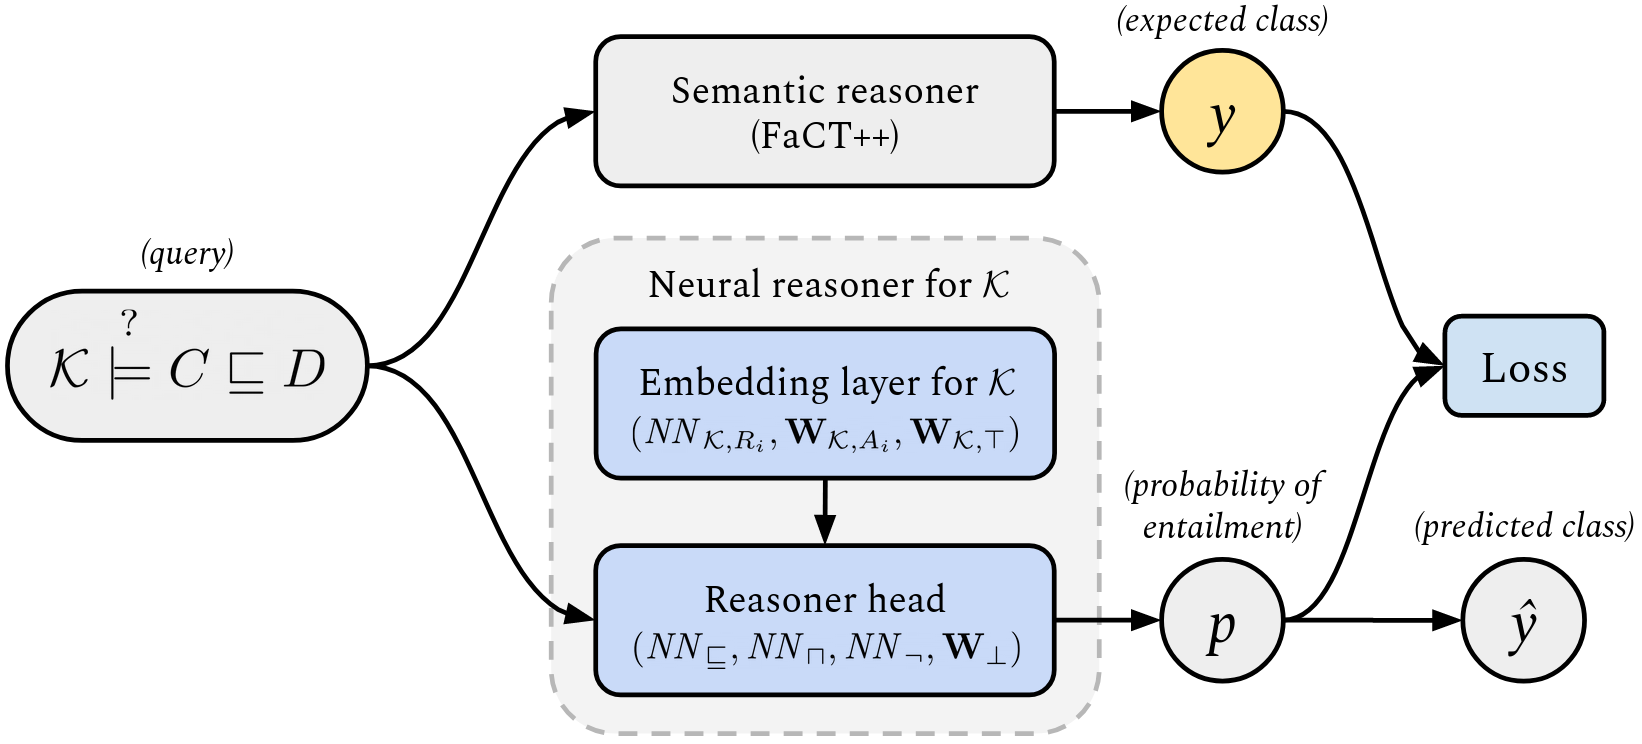
\includegraphics[width=\linewidth]{figures/reasoner.png}
\caption{
A high-level overview of the neural reasoner architecture.
An embedding layer for knowledge base $\KB$ and a reasoner head are combined to create a neural reasoner for $\KB$.
The reasoner predicts whether $\KB$ entails subsumption axioms, written $\KB \models C \sub D$, where $C$ and $D$ are $\ALC$ concepts.
We train the reasoner by contrasting the predicted probability of entailment with the answer provided by a semantic reasoner.
The reasoner head generalizes across all $\ALC$ knowledge bases, but for each $\KB$ we have to train a separate embedding layer.
The reasoner head may be frozen while training an embedding layer for a new knowledge base $\KB$, to make learning faster.
}
\label{fig:reasoner}
\end{figure}

Our deep neural reasoner (hereafter, \emph{reasoner}) is a classifier, which given a subsumption axiom, outputs the probability that the axiom is entailed by a given knowledge base.
The reasoner consists of the generic \emph{reasoner head}, and an interchangeable \emph{embedding layer} specific to a given given knowledge base.
The generic reasoner head can classify entailment, and construct embeddings for concept complements and intersection of concepts.
While an embedding layer contains embeddings for a given knowledge base -- that is, it stores embedding vectors for concept names and can construct embeddings for existential restrictions for a given role name.
A diagram of the architecture of our deep neural reasoner is shown in~\autoref{fig:reasoner}.

The main purpose of the classifier is to facilitate the computation of the gradient of the loss function with respect to the weights of the embedding layer.
In other words, when the reasoner is given an axiom, it builds its representation bottom-up from the KB-specific embeddings in the embedding layer.
That representation is then used by a neural network in the reasoner head to classify whether the axiom is entailed by that KB.
The classification output is contrasted with the target output computed by a semantic reasoner, and the value of the loss function is used to adjust weights of the embedding layer with backpropagation through structure~\cite{goller_learning_1996}.

Remember that even though we try to train the best classifier possible, the goal of the entailment classifier is learning good concept embeddings, and the resulting neural reasoner is a useful byproduct.

\subsection{Reasoner head}

In our work we chose the reasoner to be an entailment classifier for subsumption axioms in $\ALC$ -- that is, given an axiom $C \sub D$, the reasoner head outputs the probability that the axiom is entailed by a given knowledge base $\KB \models C \sub D$.
We identified integrating the ABox into reasoning as out-of-scope, so assuming that $\calA$ is empty, $\KB \models C \sub D$ holds iff $\calT \models C \sub D$ holds.

Assume that $h_\KB$ is a function mapping $\ALC$ concepts in knowledge base $\KB$ to embedding vectors in real vector space $\Real^{N_e}$, where $N_e$ is the embedding dimension.

The classification output for an entailment query $P(\KB \models C \sub D) \in (0, 1)$ (see~\autoref{eq:reasoner}) is defined as the output of the feedforward neural network $\nn_\sub$, which accepts an \emph{interaction map} of the embeddings $h_\KB(C)$ and $h_\KB(D)$, and has a single output neuron with the sigmoid activation function.
In our experiments, $\nn_\sub$ also has one hidden layer with 16 neurons, which is followed by the ELU activation function~\cite{clevert_fast_2016}.
Additional hidden layers may be added, or the number of neurons per layer may be increased if one so wishes.

\begin{equation}
\label{eq:reasoner}
    P(\KB \models C \sub D) = \sigma(\nn_\sub(h_\KB(C), h_\KB(D)))
    %P(\KB \models C \sub D) = \sigma(\nn_\sub(\nnimap(h_\KB(C), h_\KB(D))))
\end{equation}

An interaction map of a pair of embedding vectors $\nnimap(e_C, e_D)$, as defined by~\autoref{eq:interaction-map}, is a concatenation of the embedding vector $e_C$, the embedding vector $e_D$ and their outer product $e_C \otimes e_D$.
Each element of the outer product of two vectors $(\mathbf u \otimes \mathbf v)_{ij}$ is defined as $\mathbf u_i \cdot \mathbf v_j$.
Before concatenation, the outer product is reshaped to a row vector.

\begin{equation}
\label{eq:interaction-map}
    \nnimap(e_C, e_D) = [ e_C; e_D; \nnflatten(e_C \otimes e_D) ]
\end{equation}

Initially, $\nn_\sub$ simply accepted the concatenation of embeddings $h_\KB(C)$ and $h_\KB(D)$.
However, we found that a small neural network was unable to learn to classify entailment even for the simplest axioms, like $A_i \sub A_j$, where $A_i$ and $A_j$ are concept names.

We suspected that our classifier had problems learning to classify entailment because it was unable to capture pairwise correlations between embedding dimensions.
We researched possible solutions and found that using the outer product to create an interaction map between embedding vectors helps neural networks learn high-order correlations~\cite{he_outer_2018,bednarek_robustness_2020}.

In our case, adding the outer product between embeddings to the classifier inputs, allowed even a small network to perfectly memorize a training data set consisting only of entailment queries for these simple axioms, when it could not do so with a simple concatenation of embeddings.

It must be pointed out that the reasoner head does not explicitly use terminological axioms for entailment classification.
Instead, the terminological axioms indirectly shape the learned concept embeddings, so even though it may look like the reasoner head is simply memorizing answers, some form of deductive reasoning is actually performed.


\subsection{Embedding layer}

Recursive neural networks have been successfully used for encoding expression trees as fixed-size vectors, that could be used as inputs to machine learning models~\cite{goller_learning_1996}.
The recursively defined DL concepts also have a tree structure~\cite{lawrynowicz_discovery_2018}, so it is appropriate to use a recursive neural network as the embedding layer in our reasoner architecture.
The key hypothesis that defines our reasoner is that for each KB, we can train an embedding layer that embeds concepts from that KB in an embedding space with a topology that makes it easy for the reasoner head to classify entailment.
An embedding topology that is beneficial to entailment classification is formed by jointly training the reasoner head and embedding layers for multiple KBs, which forces the embedding head to generalize, and the embedding layers to output embeddings in the shared embedding space.

In general, concept embeddings are represented by vectors in real vector space $\Emb$, where $N_e$ is the embedding dimension.
We now define the function $h_\KB : \ALC \rightarrow \Emb$ that maps $\ALC$ concepts for knowledge base $\KB$ to embedding vectors in real vector space $\Emb$.

To obtain the embedding for the complement of a given concept, one first recursively obtains the embedding of that concept, and then passes it as an input to the \emph{complement constructor network} $\nn_\lnot$.
The complement constructor network is a two-layer neural network, with $N_e$ input neurons and $N_e$ output neurons with the $\tanh$ activation function.

To obtain the embedding for an intersection of concepts, one first recursively obtains the embeddings of the two concepts, computes the interaction map for these embeddings, and passes it as the input to the \emph{intersection constructor network} $\nn_\dland$, that maps the interaction map of two concept embeddings, to the embedding of their intersection.
The function $\nn_\sqcap$ is a two-layer neural network, with $2N_e + N_e^2$ input neurons (because an interaction map is a concatenation of two embeddings of size $N_e$, and of their flattened outer product, which has size $N_e^2$), and $N_e$ output neurons, followed by the $\tanh$ activation function.

To obtain the embedding for an existential restriction, one first obtains the embedding of the given concept, and passes it to the \emph{existential restriction constructor network} $\nn_{\KB,R_i}$.
The existential restriction constructor network is an a two-layer network, with an input layer with $N_e$ neurons, and an output layer with $N_e$ neurons followed by the $\tanh$ activation function.

\begin{figure}
\centering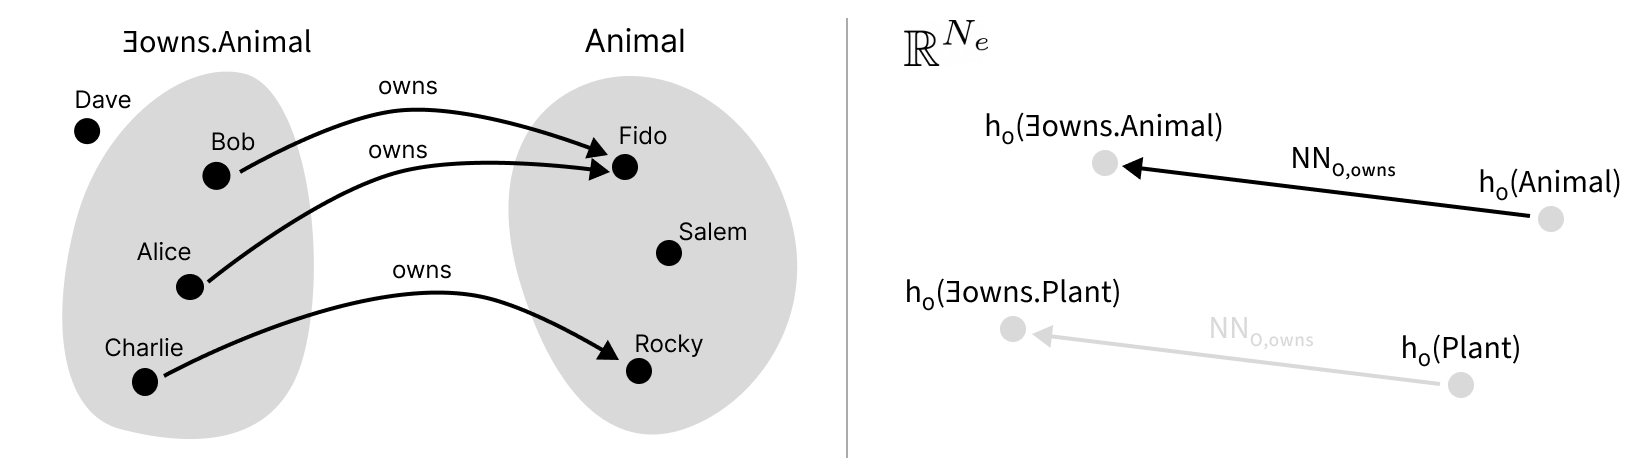
\includegraphics[width=\linewidth]{figures/role.png}
\caption{
An example interpretation of a knowledge base with role assertions is shown on the left side.
The individuals \tw{Fido}, \tw{Salem}, and \tw{Rocky} are elements of the set $\tw{Animal}^\calI$.
Individuals \tw{Alice}, \tw{Bob}, and \tw{Charlie} are elements of set $(\exists \tw{owns} . \tw{Animal})^\calI$.
An illustration of transformations from concept embeddings to existential restriction embeddings is shown on the right side.
The embedding of $\exists \tw{owns} . C$ may be obtained by applying $\nn_{\KB,\tw{owns}}$ to the embedding of concept $C$.
}
\label{fig:role}
\end{figure}

To understand the intuition behind this choice consider the following example.
On the left side of~\autoref{fig:role} we show an interpretation of a KB with a set of human individuals, and a set of individuals that are instances of concept \tw{Animal}.
Some individuals own an animal, which is described with role assertions $\tw{owns}(\tw{Alice}, \tw{Fido}), \tw{owns}(\tw{Bob}, \tw{Fido}), \tw{owns}(\tw{Charlie}, \tw{Rocky})$ (shown as arrows).
\tw{Alice}, \tw{Bob} and \tw{Charlie} may be described as instances of $\exists \tw{owns} . \tw{Animal}$.
Notice that if we reversed all \tw{owns} arrows, then an \tw{owns} arrow would always start in set \tw{Animal}, and end in set $\exists \tw{owns} . \tw{Animal}$.
By definition $(\exists R . C)^\calI = \{ x \in \dldomain \mid \exists_{y \in \dldomain} ( (x, y) \in R^\calI \land y \in C^\calI ) \}$, all elements of $(\exists R . C)^\calI$ are related to some element of $C^\calI$.
So in general, if we interpret role assertions as arrows, for any interpretation $\calI$, if we reverse role $R_i$ arrows, they always begin in set $C^\calI$ and end in set $(\exists R_i . C)^\calI$.
Now consider the right side of the figure.
Our embedding layer represents concepts as points in the embedding space $\Emb$ and does not support individuals at all, so we ``squish'' the sets $\exists \tw{owns} . \tw{Animal}$ and \tw{Animal} into points in $\Emb$, but we keep the (reversed) arrows, since their start and end points always occur inside the sets.
Because of our previous observation about roles, we think that it is appropriate to model the existential restriction constructor as a function mapping concept embeddings $h_\KB(C)$ to embeddings of the existential restriction $h_\KB(\exists R_i . C)$.
%Intuitively, the embeddings of concept $\exists R_i . C$ should occupy their own region of the embedding space.
Functions $\nn_{\KB,R_i}$ need to be learned per knowledge base $\KB$, because different KBs have different numbers of roles, and roles may have different meanings, so there is no obvious way of sharing existential restriction constructors between KBs.

The embedding for each concept name $A_i$ is simply stored in a vector $\bfW_{\KB,A_i}$ of dimension $N_e$. The concept name embeddings are KB-specific, since different KBs have a different number named concepts with different meanings.

The embedding of the top concept is stored as an KB-specific vector $\bfW_{\KB,\top}$, because the most general concepts in a given KB should be close to the top concept in the embedding space, but depending on the vocabulary it might make sense for these general concepts to occupy a different region of the embedding space.

The embedding of the bottom concept is stored by the vector $\bfW_\bot$. We do not see a reason to make the embedding of the bottom concept $\bfW_\bot$ dependent on the KB.

To ensure that we do not combine multiple linear transformations, the outputs of the constructor networks are followed by the $\tanh$ activation function.
To keep concept embedding values in the same range, regardless of whether the input concept was a concept name, top concept, bottom concept, or a concept expression, we also apply the $\tanh$ function to $\bfW_{\KB,A_i}$, $\bfW_{\KB,\top}$, and $\bfW_{\bot}$.

\begin{equation}
\label{eq:restricted-encoder}
\begin{split}
    h_\KB(\lnot C) &= \tanh \nn_{\lnot}(h_\KB(C)) \\
    h_\KB(C \dland D) &= \tanh \nn_{\dland}(\nnimap(h_\KB(C), h_\KB(D))) \\
    h_\KB(\exists R_i . C) &= \tanh \nn_{\KB,R_i}(h_\KB(C)) \\
    h_\KB(A_i) &= \tanh \bfW_{\KB,A_i} \\
    h_\KB(\top) &= \tanh \bfW_{\KB,\top} \\
    h_\KB(\bot) &= \tanh \bfW_{\bot}
\end{split}
\end{equation}

It is not necessary for the embedding layer to support the constructors for concept unions, and universal restrictions.
Since the de Morgan laws hold in $\ALC$, one can express concept union in terms of concept complement and intersection.
One can also use the quantifier negation law to express universal restrictions in terms of concept complement and existential restrictions~\cite{rudolph_foundations_2011}.

\begin{equation}
\label{eq:alc-demorgan}
\begin{split}
C \dlor D &\equiv \lnot (\lnot C \dland \lnot D) \\
\forall R . C &\equiv \lnot \exists R . \lnot C
\end{split}
\end{equation}

Using the above equivalences, we define the embeddings for concept unions and universal restrictions as follows.

\begin{equation}
\label{eq:encoder-cheats}
\begin{split}
    h_\KB(C \dlor D) &= h_\KB(\lnot (\lnot C \dland \lnot D)) \\
    h_\KB(\forall R_i . C) &= h_\KB( \lnot \exists R_i . \lnot C )
\end{split}
\end{equation}

\subsection{Relaxed architecture}
\label{sec:restricted}

It is important to note that in the embedding layer, that we introduced in the previous section, the weights of the neural networks $\nn_\lnot$ and $\nn_\dland$ are not dependent on a specific knowledge base.
Since the semantics of concept complement and intersection constructors do not change depending on a KB, we think that their neural equivalents should also not change.
We call a reasoner, where $\nn_\lnot$ and $\nn_\dland$ network weights are stored in the reasoner head the \emph{restricted reasoner}.
Unless stated otherwise, we use restricted reasoners.

However, we did initially experiment with a variant of the reasoner, that allows the embedding layer to learn KB-specific concept constructor networks $\nn_{\KB,\lnot}$ and $\nn_{\KB,\dland}$, and a KB-specific embedding of the bottom concept $\bfW_{\KB,\bot}$.
We call this variant the \emph{relaxed reasoner}.
All changes to the function $h_\KB$ in the relaxed reasoner are marked below in red.

\begin{equation}
\label{eq:relaxed-encoder}
\begin{split}
    h_\KB(\lnot C) &= \tanh \nn_{\textcolor{red}{\KB},\lnot}(h_\KB(C)) \\
    h_\KB(C \dland D) &= \tanh \nn_{\textcolor{red}{\KB},\dland}(\nnimap(h_\KB(C), h_\KB(D))) \\
    h_\KB(\bot) &= \tanh \bfW_{\textcolor{red}{\KB},\bot} \\
\end{split}
\end{equation}

In the relaxed architecture, the only weights shared between different KBs are the ones learned by the classifier $\nn_\sub$, which we expected would allow the embedding layers to learn more fitting embeddings, at the cost of limiting generalization and opportunities for transfer learning.


\subsection{Training procedure}

The training procedure for our reasoner consists of two steps.

In the first step we train both the reasoner head and embedding layers for as many diverse KBs as possible.
This results in a reasoner head that learned to classify whether subsumption axioms hold in any KB, given that an appropriate embedding layer is provided.
By appropriate embedding layer we mean a layer that learned to embed KB-specific concepts in a space that minimizes the classifier loss.
We simply call this step \emph{training the reasoner head}, and we consider the data used in this step as the \emph{training data set}.
Note that as a result of training the reasoner, we obtain trained embedding layers for KBs in the training data set.
If obtaining the trained embedding layers was the goal, then the next step is not necessary.

In the second step, we freeze the reasoner head and train the embedding layers for KBs that were not seen in the first step.
This results in embedding layers that can embed concepts in a space in which the reasoner is good at classification.
We think that if our reasoner can accurately classify whether subsumption axioms are entailed by a KB, then the embeddings used as the input to the classifier $\nn_\sub$ faithfully capture the semantics of the KB, \emph{even though we did not train the reasoner head at all}.
We call this step \emph{training the embedding layers} or \emph{testing the reasoner head}, and we consider the data set used in this step as the \emph{test data set}.

%\begin{equation}
%\label{eq:loss}
%    \ell(y, \hat y) = - \frac{1}{n} \sum_{i=1}^n \left[ y_i\log(\hat y_i) + (1 - y_i)\log(1 - \hat y_i) \right]
%\end{equation}


\subsection{Axiom generator}
\label{sec:random_axiom}

Our reasoner learns embeddings by learning to classify entailment queries $\KB \models C \sub D$.
A set of query axioms could be created manually, but of course, learning will be successful only if a large number of subsumption axioms is provided.
One way of obtaining a large number of axioms would be to generate all possible axioms for a given KB, up to some maximum expression tree depth.
This approach would suffice for shallow expression trees and KBs with very small vocabularies, but is impractical otherwise.
A more practical method of obtaining a large set of axioms is to pseudo-randomly generate them.
The most important advantages of pseudo-randomly generating expression trees are that it is fast and that the number of training examples is unlimited.
Another advantage is the ability to manually set the initial state of the pseudo-random number generator.
One can easily recreate a data set by setting the seed value, which makes storing data sets on disk unnecessary.
One drawback of pseudo-randomly generating training data is the possibility of generating duplicate axioms which may need to be discarded, depending on how the reasoner is trained.

One algorithm for pseudo-randomly generating $\ALC$ expressions (including axioms) was introduced by Eberhart~et~al.~\cite{eberhart_pseudo-random_2018}.
We could not use their implementation, because it uses the Java Virtual Machine, so we implemented our own custom generator inspired by their algorithm.

Our axiom generator has four parameters: the set of concept names $N_C$, the set of role names $N_R$, the probability $p_A$ of generating a concept name instead of a top or bottom concept, and the maximum depth of recursion $d_{max}$.
Expressions are generated recursively and the current recursion depth $d$ is tracked.

Axioms are generated by starting with the grammar rule $\bfA$ (\autoref{eq:alc-axiom-grammar}), which returns a subsumption axiom or a disjointness axiom with equal probability.
The second alternative is intentionally redundant, because disjointness axioms were generated too rarely without it, even though they are common in real-world KBs (generating more disjointness axioms helped us achieve good results in~\autoref{chap:casestudy}, where the analyzed KB had many disjoint concepts).
Regardless of which alternative was returned, two concepts are generated according to grammar rule $\bfC$ (\autoref{eq:alc-concept-grammar}).
The maximum depth of recursion for the first concept $d_{max,1}$ is chosen from the uniform discrete distribution $\mathcal{U}\{1, d_{max}\}$, and the maximum depth of recursion for the second concept $d_{max,2}$ is chosen from $\mathcal{U}\{1, \max\{1, d_{max} - d_{max,1} \} \}$.
This technique of limiting the expression depth results in axioms where one of the concepts is deeper than the other, or axioms where both concepts are relatively shallow.
If both concepts in an axiom are deep, then inference can be very slow in \factpp{}, which is problematic when computing answers for tens of thousands of axioms.

\begin{equation}
\label{eq:alc-axiom-grammar}
\bfA \Coloneqq \bfC \sub \bfC \mid \bfC \dland \bfC \sub \bot
\end{equation}

The grammar rule $\bfC$ returns one of the following alternatives with equal probability: a concept according to grammar rule $\bfT$ (\autoref{eq:alc-terminal-grammar}), a concept complement, a concept intersection, a concept union, an existential restriction or a universal restriction.
For existential and universal restrictions, the role name $R_i$ is chosen randomly from $N_R$, with equal probability for each role name.
If the recursion depth is equal to or greater than $d_{max}$, then a concept according to grammar rule $\bfT$ is always returned.

\begin{equation}
\label{eq:alc-concept-grammar}
\bfC \Coloneqq \bfT \mid \lnot \bfC \mid \bfC \dland \bfC \mid \bfC \dlor \bfC \mid \exists R_i . \bfC \mid \forall R_i . \bfC
\end{equation}

The $\bfT$ grammar rule returns one of the following alternatives: with probability $p_A$, a concept name $A_i$ chosen uniformly at random from $N_C$, the top concept with probability $\frac{1 - p_A}{2}$, or the bottom concept with probability $\frac{1 - p_A}{2}$.
It is crucial that the probability of returning $\top$ or $\bot$ does not depend on the number of concept names $|N_C|$.

\begin{equation}
\label{eq:alc-terminal-grammar}
\bfT \Coloneqq A_i \mid \top \mid \bot
\end{equation}

\section{Experiment 1 -- Transfer test}

To test our reasoner we first examine the ability of the reasoner head to correctly predict whether a KB entails subsumption axioms, and by extension, how good are the embeddings learned by the embedding layer.

Then we test if a reasoner head trained on KBs in the training data set, generalizes to unseen KBs from the test data set.
The transfer test is described in the next section.

In this experiment we examine both the relaxed reasoner architecture and the restricted reasoner architecture, and compare the advantages and disadvantages of the two variants.

\subsection{Transfer test}

We designed a simple test to check whether a trained reasoner head actually learns to reason in the $\ALC$ description logic, and high classification metric values are not just the effect of embedding layers overfitting to KBs.

We test our architecture by first training the reasoner head and embedding layers on the training data set (as usual), which results in a skillful reasoner.
Then we create a no-skill reasoner head, that is not trained, but only randomly initialized.
For each of the two reasoner heads, we train embedding layers on the test data set, but keep the reasoner head weights frozen.
After training the embedding layers on the test data set for a set number of epochs, if the classification metrics for the reasoner with the trained head are significantly greater than for the reasoner with the random head, then the trained reasoner head learned useful relations in the $\ALC$ embedding space that generalize to new KBs.
In short, the reasoner head is transferable.

Conversely, if the differences between classification metrics of both reasoner heads are not significant, then the trained reasoner actually has little or no skill, and the only skill in classification comes from the embedding layer, which would mean that the reasoner head is not transferable.

\subsection{Synthetic data set}

Finding a large number of $\ALC$ KBs with a small number of concept and role names proved difficult, so for this experiment we generated a synthetic data set.

The data set for this consists of 60 randomly generated KBs.
We wanted the KBs to be non-trivial, so the number of concept names $|N_C|$ for each KB is chosen randomly from the discrete uniform distribution $\calU \{ 80, 120 \}$, and the number of role names $|N_R|$ is chosen randomly from the discrete uniform distribution $\calU \{ 1, 5 \}$.
The number of role names is very small, because we observed that the number of role names in real-world KBs is typically much smaller than the number of concept names.
The actual concept and role names are simply ordinal numbers, and are not considered in any way during learning.

For each KB we also randomly choose the number of terminological axioms $|\calT|$ to generate, from the normal distribution $\lfloor \calN(200, 10) \rfloor$.
We decided that the average number of axioms per KB should be about 2 times bigger than the number of concept names, but should vary a bit.
That said, the number of axioms should not be too small nor too big, because when we generate entailment queries later, the probability of randomly generating an axiom entailed by a KB would be too big for KBs with a small proportion of axioms per concept name, or too small for KBs with a large number of axioms per concept name, and that would lead to a strong class imbalance, which is of course undesirable.

Terminological axioms are randomly generated according to the procedure that we described in~\autoref{sec:random_axiom}.
We set the maximum depth of axioms $d_{max}$ to 3, because we wanted to keep axioms simple, and thus more general, and with more influence on the interpretation of the KB.
The parameter $p_A$ is chosen randomly for each KB from the uniform distribution $\calU [0.9, 1]$, as the probability of $\top$ and $\bot$ in a concept expression should be low.

Every time a new axiom is generated for a KB we test if adding it to $\calT$ would make the KB inconsistent or if it would make more than 10\% of named concepts unsatisfiable (unsatisfiable concepts do occur in real-world KBs, but reasoning in KBs with too many unsatisfiable concepts would be too easy, so we set an upper limit).
If so, the problematic axiom is discarded, and we try generating a new axiom.

For each knowledge base $\KB$ we additionally generate 2000 unique random queries $\KB \models \alpha$, where $\alpha$ is a random subsumption axiom.
The same parameters of the random axiom generator are used, as during generating terminological axioms for that KB.
For each query we perform the entailment check $\KB \models \alpha$ with \factpp{}.
If the KB entails $\alpha$, then the expected class of the query is set to $y = 1$.
Otherwise the expected class of the query is set to $y = 0$.

After generating KBs and their query sets, we split the data set into the training data set and the test data set.
The first 40 KBs and their queries are assigned to the training data set, and the last 20 KBs and their queries are placed in the test data set.
We then create a validation data set from 20\% of the queries from the training data set.
In total, there are $64 000$ queries in the training data set, $16 000$ queries in the validation data set, and $40 0000$ queries in the test data set.
In every data set, approximately 21.5\% of queries have class $y = 1$ and the remaining queries have class $y = 0$.
This class imbalance does not significantly affect our experiments, so we do not use any methods for dealing with imbalanced data sets.

KB parameters are sampled from probability distributions instead being set to constant values, to reduce bias in the data set.
We do admit that we parameterized the probability distributions mostly according to our intuition, so perhaps a harder data set could be created.
However, in retrospect, we think that the data set was hard enough to provide some challenge for reasoners in our experiments.

The data set can be reproduced by setting the initial state of the random number generator to a value specified in the attached code.

\subsection{Training details}

The embedding dimension is set to $N_e = 10$, which is a much smaller number than $|N_C|$.
This forces the embeddings for different concept names to share embedding dimensions.

As the loss for our classifier we use binary cross entropy.
We create one AdamW optimizer~\cite{loshchilov_decoupled_2019} per reasoner head with learning rate set to $\eta_c = 0.0001$, and one AdamW optimizer per embedding layer with learning rate set to $\eta_e = 0.0002$.
The AdamW optimizer was the first optimizer we tested, and learning progressed smoothly, so we did not see the need to change it.
The learning rates were tuned manually.
In total, for each reasoner variant we create 1 optimizer for the reasoner head, and 60 optimizers for the embedding layers. 

We train both reasoner variants with mini-batch gradient descent for 15 epochs, which was enough for the validation loss to stop decreasing.
During testing, we train the embedding layers (while the reasoner head is frozen) for 10 epochs, as the test loss stabilized after that.
We set the batch size to 32, as small batch sizes have been shown to improve generalization~\cite{masters_revisiting_2018}. 

Unless stated otherwise, all weights are randomly initialized using the Xavier initialization~\cite{glorot_understanding_2010}.

\subsection{Evaluation metrics}

Even though the quality of the embeddings learned by the embedding layer cannot be measured directly, we can still compute classification metrics for a trained reasoner.
As mentioned, we think that if the classification metrics indicate good performance, then the embeddings learned by the embedding layer must capture the semantics of a given KB well.
If that was not the case and the embeddings did not encode useful information for inference in the $\ALC$ DL, then the classifier should not be able to reliably classify entailment of axioms.

Our classifier learns binary classification, so we chose appropriate metrics~\cite{tharwat_classification_2021}.
Firstly, we include accuracy (\autoref{eq:metric-accuracy}) in the set of evaluation metrics.
Because the data set that we generated for the experiments is slightly imbalanced we also compute precision (\autoref{eq:metric-precision}), recall (\autoref{eq:metric-recall}), and the F1-score (\autoref{eq:metric-f1}). 

For simplicity, in threshold-sensitive metrics we choose a threshold of 0.5.
In other words, for query $\KB \models \alpha$, if the probability of entailment according to the reasoner is greater than the threshold $P(\KB \models \alpha) \geq 0.5$, then the predicted class for the query is $\hat y = 1$.
Otherwise, the predicted class is $\hat y = 0$.
Given that $y$ is the expected class, in the equations below, TP is defined as the number of true positives (number of queries, where $\hat y = y = 1$), TN is the number of true negatives (number of queries, where $\hat y = y = 0$), FP is the number of false positives (number of queries, where $\hat y = 1$ and $y = 0$), and FN is the number of false negatives (number of queries, where $\hat y = 0$ and $y = 1$).

\begin{equation}
\label{eq:metric-accuracy}
\text{Accuracy} = \frac{\text{TP} + \text{TN}}{\text{TP} + \text{TN} + \text{FP} + \text{FN}}
\end{equation}

\begin{equation}
\label{eq:metric-precision}
\text{Precision} = \frac{\text{TP}}{\text{TP} + \text{FP}}
\end{equation}

\begin{equation}
\label{eq:metric-recall}
\text{Recall} = \text{TPR} = \frac{\text{TP}}{\text{TP} + \text{FN}}
\end{equation}

\begin{equation}
\label{eq:metric-f1}
\text{F1} = \frac{2 \cdot \text{Precision} \cdot \text{Recall}}{\text{Precision} + \text{Recall}}
\end{equation}

Additionally, we visualize the receiver operating characteristic (ROC) curve, the precision-recall (PR) curve, and the confusion matrix (the number for each cell of the confusion matrix is normalized by dividing it by the total number of samples in the data set).
The ROC curve shows the performance of a classification model at all classification thresholds, by plotting the true positive rate (TPR; also called recall) against  the false positive rate (FPR) (\autoref{eq:metric-fpr}).
Similarly, the PR curve shows the performance of a model at all thresholds, but by plotting precision against recall~\cite{saito_precision-recall_2015}.
For both ROC and PR curves, larger area under the curve suggest a better classifier.

We also compute the value of the area under the ROC curve (AUC ROC), which is a threshold-invariant metric with a minimum value of 0 and a maximum value of 1.
Higher AUC ROC values indicate better classification performance~\cite{fawcett_introduction_2006}.

\begin{equation}
\label{eq:metric-fpr}
\text{FPR} = \frac{\text{FP}}{\text{FP} + \text{TN}}
\end{equation}

The test data set contains 20 KBs, with 2000 queries for every KB.
We compute all metrics separately for each query set, and then compute the average and standard deviation across KBs.
In the case of the ROC and PR curve plots, in addition to plotting the curves for each query set, we also plot the averaged curves.   
We do this because the KBs in the test data set may be unequally difficult to classify, so it is beneficial to measure the variance of the reasoner performance across different KBs.

We think that together, AUC ROC, accuracy, precision, recall, F1-score, ROC analysis, PR analysis, and confusion-matrix analysis should provide an accurate image of the performance of the evaluated reasoners.


\subsection{Evaluation of reasoning ability}

We evaluate the reasoning ability of our reasoner by monitoring the training and validation loss and AUC ROC values during training.
The only goal of this assessment is to verify that the reasoner can effectively learn to classify entailment in the training data set, and does not suffer from underfitting.
Training and validation losses steadily decreasing, and validation AUC ROC increasing with each training epoch, suggests that the reasoner architecture is sufficient for learning to classify entailment in a given data set.

\begin{figure}
\makebox[\textwidth][c]{
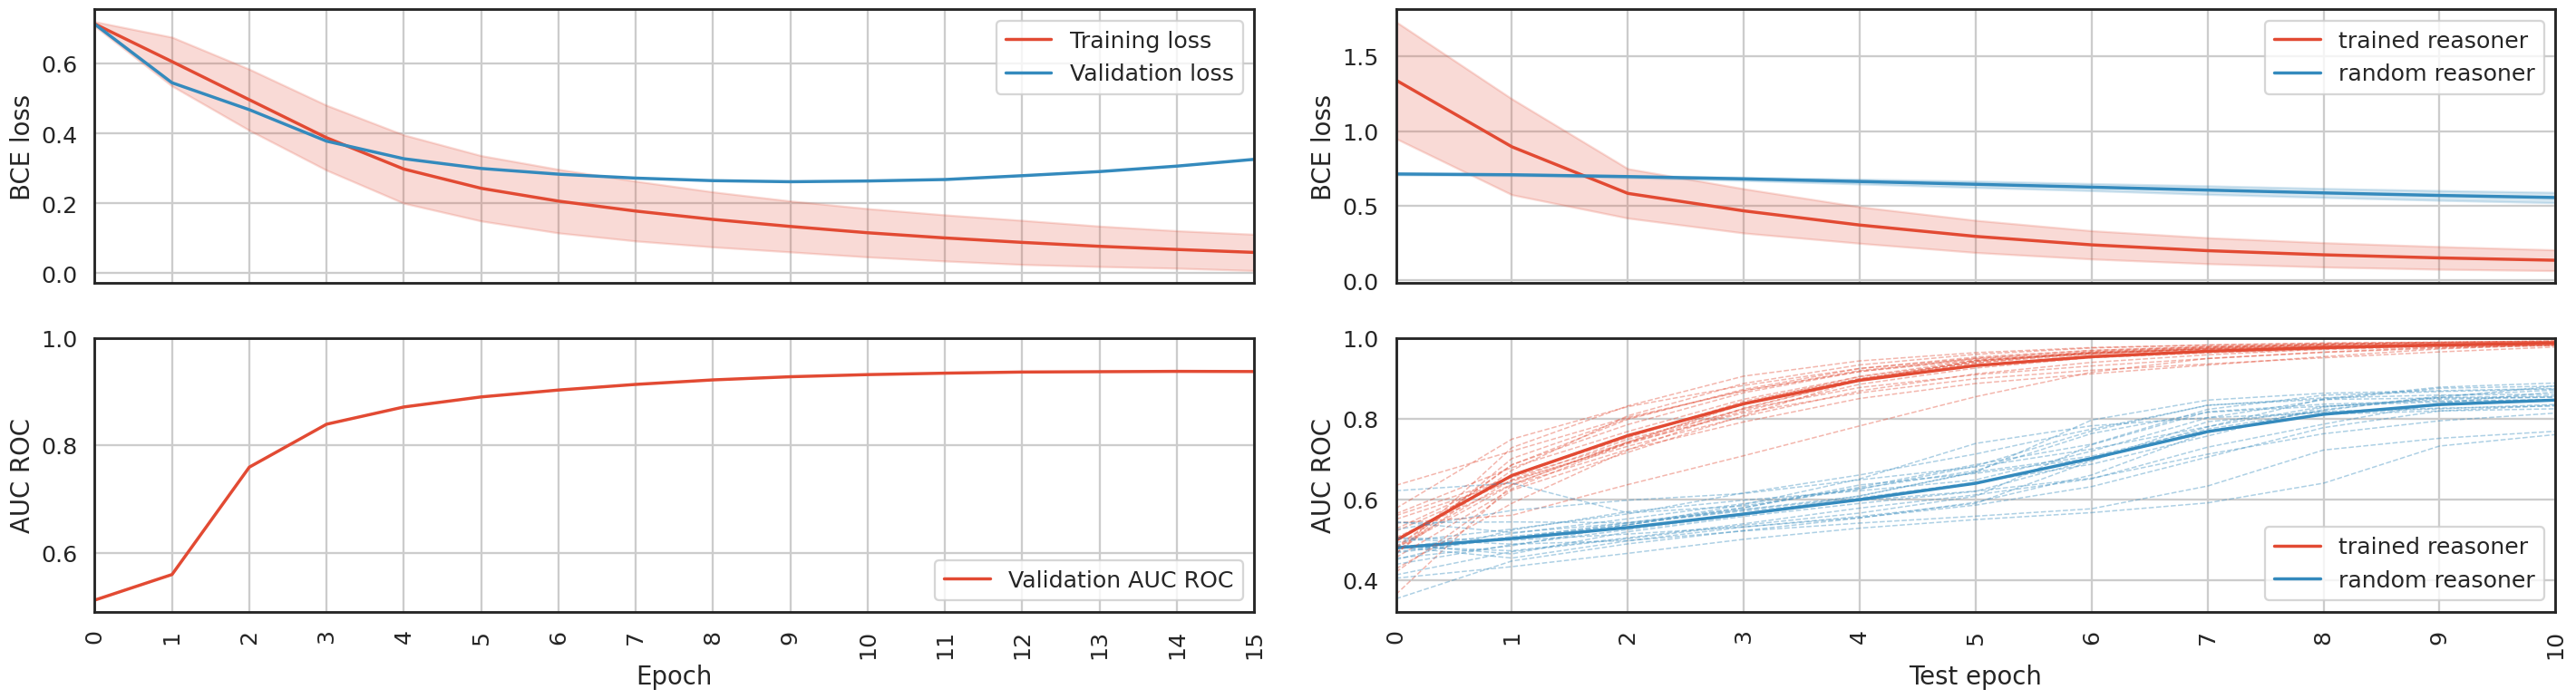
\includegraphics[width=1.15\linewidth]{figures/ex1-progress.png}
}
\centering
\caption{
Training and test progress of the relaxed reasoner.
The reported training loss for each epoch is the average mini-batch loss in that epoch.
We also show the standard deviation of the mini-batch loss for each epoch.
In test progress, the trained reasoner is shown in red, while the random reasoner is shown in blue.
The reasoner was \emph{not} trained during epoch 0 of training and testing -- during epoch 0 we only compute the initial loss and metric values.
Dashed lines show the AUC ROC for each KB in the test data set, while the thicker blue and red curves are the averaged AUC ROC across KBs in the test data set.
}
\label{fig:ex1-progress}
\end{figure}

\begin{figure}
\makebox[\textwidth][c]{
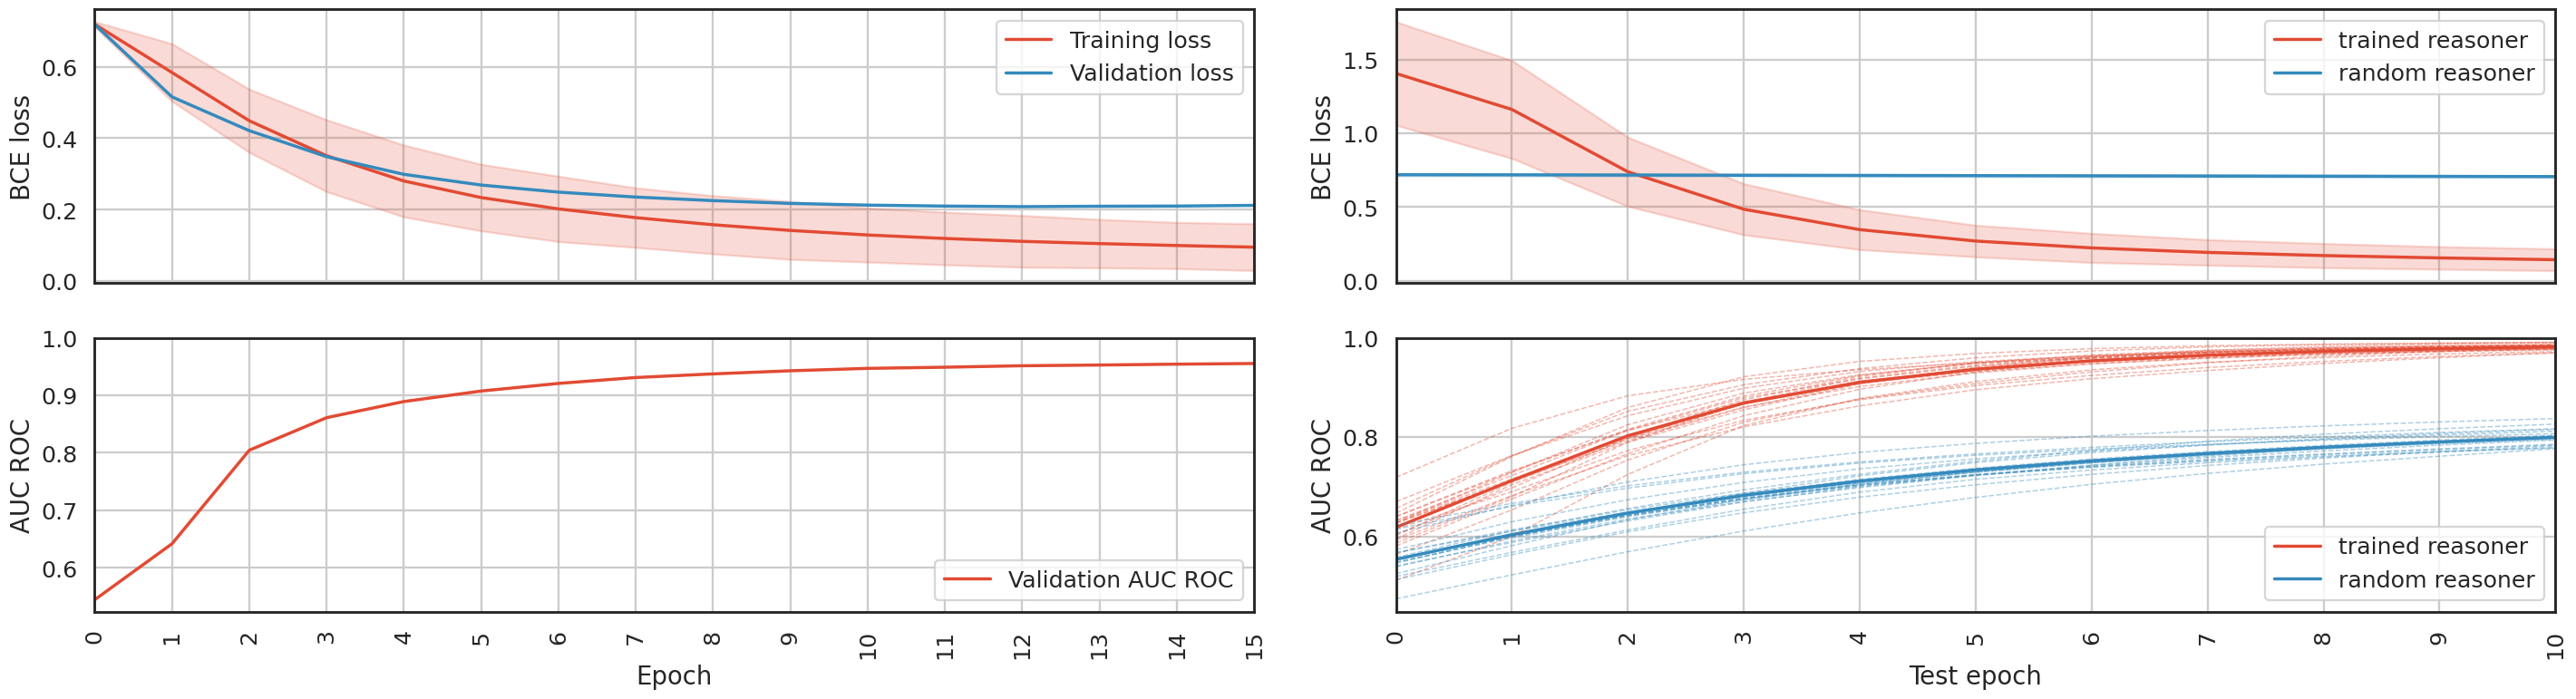
\includegraphics[width=1.15\linewidth]{figures/ex2-progress.png}
}
\centering
\caption{
Training and test progress of the restricted reasoner.
Note that the random reasoner loss actually decreases, but a very slow rate.
}
\label{fig:ex2-progress}
\end{figure}

First, we trained the relaxed reasoner on the training data set.
The training progress for this variant is shown in~\autoref{fig:ex1-progress}.
The training loss decreases and the validation AUC ROC increases for the entirety of the training, with smaller gains after epoch 10.
The validation loss decreases until epoch 10, and then start increasing, which indicates overfitting.

As shown in~\autoref{fig:ex2-progress}, the AUC ROC metric for the validation set increases when training the restricted reasoner, and does so even faster than when training the relaxed reasoner.
We attribute the faster convergence to the shared concept constructor networks $\nn_\lnot$, $\nn_\dland$, which effectively have $n$ times more training samples, where $n$ is the number of training KBs, because they are trained on every sample from every KB, compared to the relaxed architecture, in which KB-specific concept constructor networks are trained on samples from one KB.
Furthermore, the validation loss does not start increasing in later epochs, which suggests that the restricted reasoner variant is less prone to overfitting than the relaxed reasoner.
The constraint that the concept constructor networks must be the same for each KB does not lower the classification metrics much, while leading to better generalization by virtue of constructors not being KB-dependent.

In this experiment our reasoner (in both variants) was able to learn on the training data set, without extensive hyperparameter tuning.
However, if one should notice that the reasoner is underfitting on their data set, and if tuning learning rates does not help, then one should increase the number of hidden layers, or the number of neurons per hidden layer in the $\nn_\sub$ network to make the reasoner head more powerful.
If modifying $\nn_\sub$ does not yield better results, then one should try to gradually increase the embedding dimension $N_e$, up to the maximum number of concept names for a KB in the data set.

\subsection{Evaluation of knowledge transfer}

After training the relaxed reasoner, we froze the reasoner head, and trained embedding layers on the test data set.
We also trained embedding layers in conjunction with a randomly initialized reasoner head.
The test progress is shown on the right side of~\autoref{fig:ex1-progress}.
At the beginning, the test loss for the trained reasoner head was higher than the test loss for the randomly initialized reasoner head.
The test loss decreased quickly for the reasoner with the trained head, while the loss for the random head decreased very slowly.
For the reasoner with the trained head, the test AUC ROC quickly increased to almost 0.8 after epoch 2, and approached 1 after the last epoch.
The average test AUC ROC for the random head slowly increased from around 0.5 in the beginning to around 0.6 in epoch 5.
After epoch 5, the AUC ROC for the random head had a relatively big increase to around 0.8 in the last epoch.

Overall, training embedding layers for the relaxed reasoner with the trained head was much faster, than for the reasoner with the randomly initialized head, as the reasoner with the trained head achieved average AUC ROC greater than 0.8 after epoch 3, while it took the reasoner with the random head 10 epochs to do the same.
Moreover, the trained head allowed the reasoner to achieve average AUC ROC close to 1 on the test data set after 10 epochs, while the reasoner with the random head only achieved average AUC ROC of around 0.8. 

Similarly to the relaxed reasoner, after training the restricted variant, we froze the reasoner head, and trained embedding layers on the test data set.
We also trained embedding layers in conjunction with a randomly initialized restricted reasoner head.
The test progress for the restricted reasoner is shown on the right side of~\autoref{fig:ex2-progress}.
The test loss for the restricted reasoner with the trained head decreased similarly to the relaxed reasoner with the trained head.
However, the test loss for the restricted reasoner with the randomly initialized head decreased so slowly, that the test loss curve seems stationary on the plot (we checked that the loss indeed decreased, but extremely slowly).
Even though the test loss decreased very slowly for the random head, the test AUC ROC visibly increased to about 0.8 after the last epoch, which is similar to the final result of the relaxed reasoner with the random head. 
The average AUC ROC increased very quickly for the reasoner with the trained head, achieving average AUC ROC of about 0.8 after epoch 2, more than 0.9 after epoch 5, and approaching 1 after the last epoch. 

%We conclude that, although the embedding layers can adjust to minimize the classification loss, even to a no-skill reasoner, the reasoner head that was trained on the training data can learn to generalize across KBs, which results in faster convergence and better classification metrics on unseen ontologies.
%We think that the results of the transfer experiments show, that our reasoner is indeed transferable, thanks to the reasoner head, which demonstrated the ability to learn the semantics of $\ALC$ concepts in a common embedding space.


\subsection{Comparative results}

\begin{table}
\caption{
Combined test data set metrics for the relaxed and restricted reasoners.
Metric values were averaged across different KBs in the test data set.
In addition to averages, we standard deviation values are shown.
}
\label{tab:transfer-test}
\begin{adjustwidth}{-2cm}{-2cm}
\centering
\begin{tabular}{lcccccc}
\toprule
Model              & AUC ROC & F1     & Accuracy & Precision & Recall \\
\midrule
Relaxed (trained head)    & $0.9867 \pm 0.0042$ & $0.8998 \pm 0.0172$ & $0.9572 \pm 0.0074$ & $0.9715 \pm 0.0191$ & $0.8385 \pm 0.0259$ \\
Relaxed (random head)     & $0.8461 \pm 0.0343$ & $0.6776 \pm 0.0464$ & $0.8423 \pm 0.0372$ & $0.6544 \pm 0.0773$ & $0.7131 \pm 0.0602$ \\
\midrule
Restricted (trained head) & $0.9816 \pm 0.0064$ & $0.8891 \pm 0.0219$ & $0.9525 \pm 0.0106$ & $0.9628 \pm 0.0144$ & $0.8262 \pm 0.0298$ \\
Restricted (random head)  & $0.7995 \pm 0.0164$ & $0.3876 \pm 0.0174$ & $0.2769 \pm 0.0144$ & $0.2406 \pm 0.0134$ & $0.9971 \pm 0.0024$ \\
\bottomrule
\end{tabular}
\end{adjustwidth}
\end{table}

The combined test data set metrics, that our reasoners achieved in this experiment, are shown in~\autoref{tab:transfer-test}.
We also visualize the ROC and PR curves, and confusion matrices for the test data set for the relaxed reasoner in~\autoref{fig:ex1-vs}, and for the restricted reasoner in~\autoref{fig:ex2-vs}.

As expected, for both relaxed and restricted reasoners, the reasoners with trained heads achieved superior performance on the test data set, which shows that both variants of our reasoner are indeed transferable.
For the relaxed architecture, the trained model is strictly better than the randomly initialized one, as all metric values are higher for the former.
Moreover, the trained model has lower variance of metrics across KBs in the test data set, than the random model. 
For the restricted architecture, the trained model is significantly better than the randomly initialized one on all metrics except recall.
The extremely high recall of the random reasoner is of course worthless, given its very low precision.
The restricted trained reasoner has lower variance than the restricted random reasoner for AUC ROC and accuracy.
However, the restricted random reasoner has  lower variance for F1-score, precision and recall.

Between the two random reasoners, the relaxed variant achieves better metric values, except recall, due to the very high recall of the restricted random reasoner.
This was expected, since in the relaxed variant, the complement and intersection constructor networks can adjust to the randomly classifier to minimize the classification error, while in the restricted variant this is not possible.

When comparing the trained reasoners, the relaxed variant achieves slightly higher values with lower variance for all metrics (except precision, for which the restricted variant has slightly lower variance).
We were also not surprised by these results, as we expected that sharing constructor networks between all KBs would force the reasoner to generalize, which would also increase variance in metric values for KBs in the test data set.
The restricted reasoner has a big advantage, that we think negates its slightly lower metric values and slightly higher variance in comparison to the relaxed variant -- it has less learnable parameters.

Since one of the main goals of our reasoner is transfer learning, the lower number of parameters in the embedding layer speeds up training for new KBs.
The average embedding layer training time per epoch was 21.72 seconds for the restricted variant, and 26.84 seconds per epoch for the relaxed variant, which is 23\% slower.
For the relatively simple constructor networks that we use in our work, this is not very significant, but we expect the time savings to greatly increase, when these networks are scaled-up to deal with bigger data sets and more complex KBs.

\newpage

\begin{figure}[h!]
\makebox[\textwidth][c]{
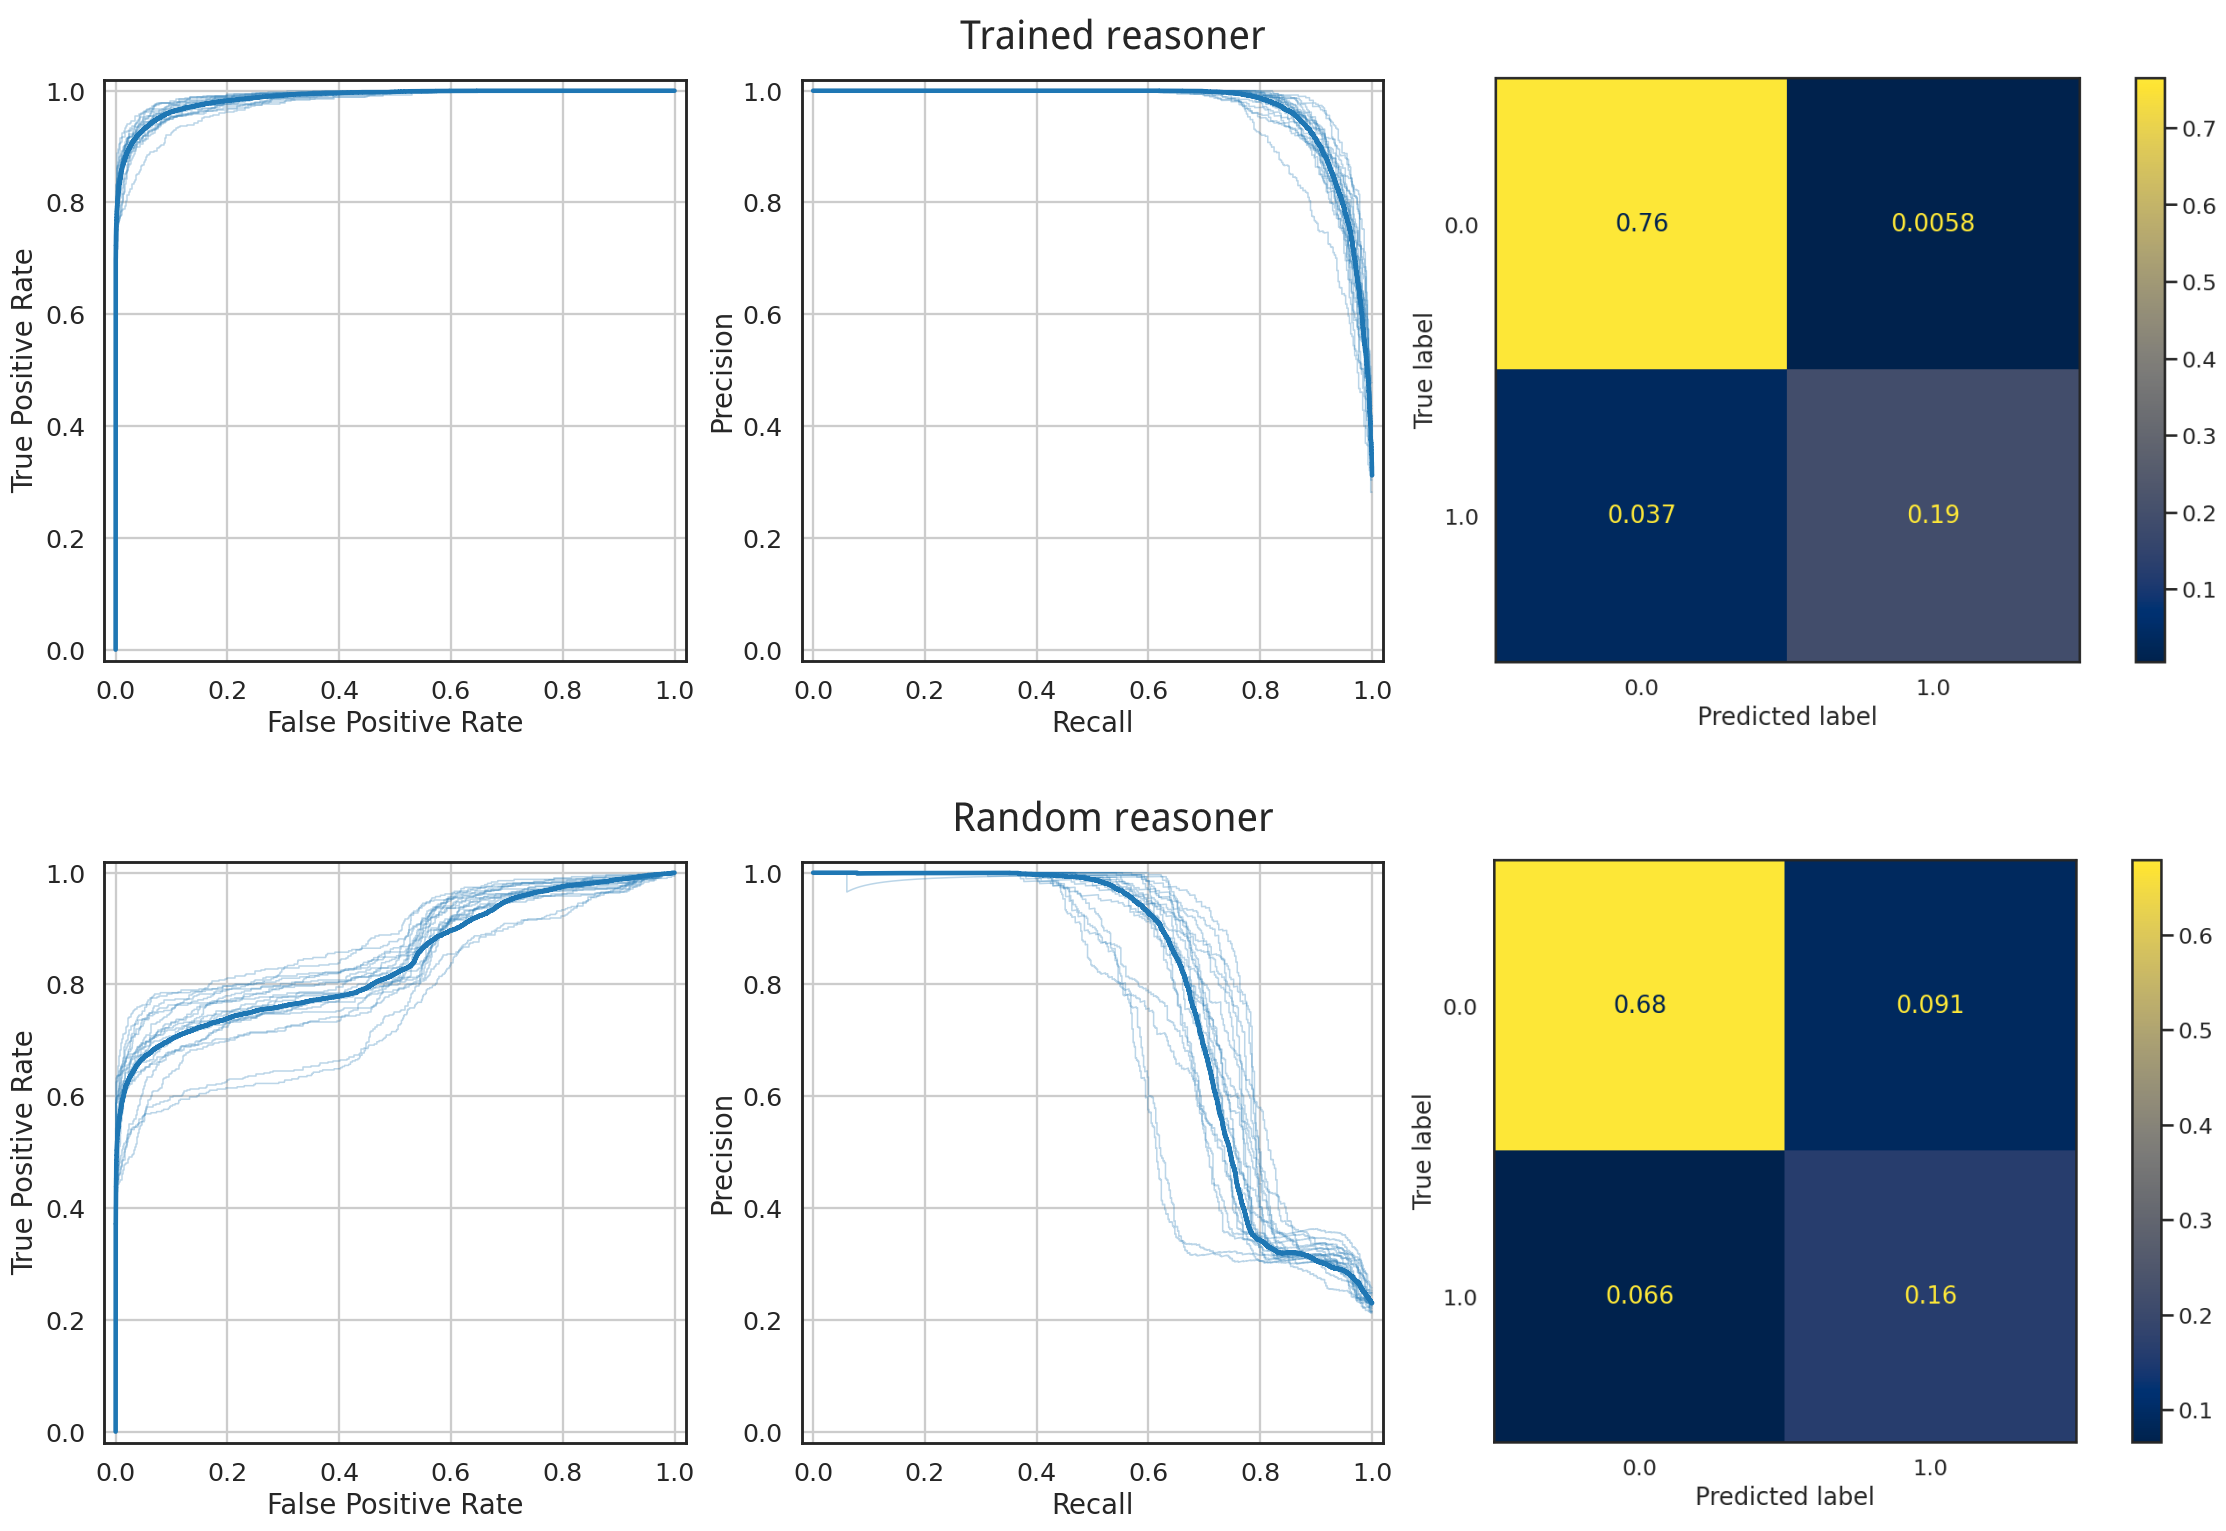
\includegraphics[width=1\linewidth]{figures/ex1-vs.png}
}
\centering
\caption{
ROC curves and confusion matrices for the relaxed reasoner.
The visualizations reflect classification performance on the test data set.
Confusion matrices are normalized by the number of all samples in the test data set.
}
\label{fig:ex1-vs}
\end{figure}

\begin{figure}[h!]
\makebox[\textwidth][c]{
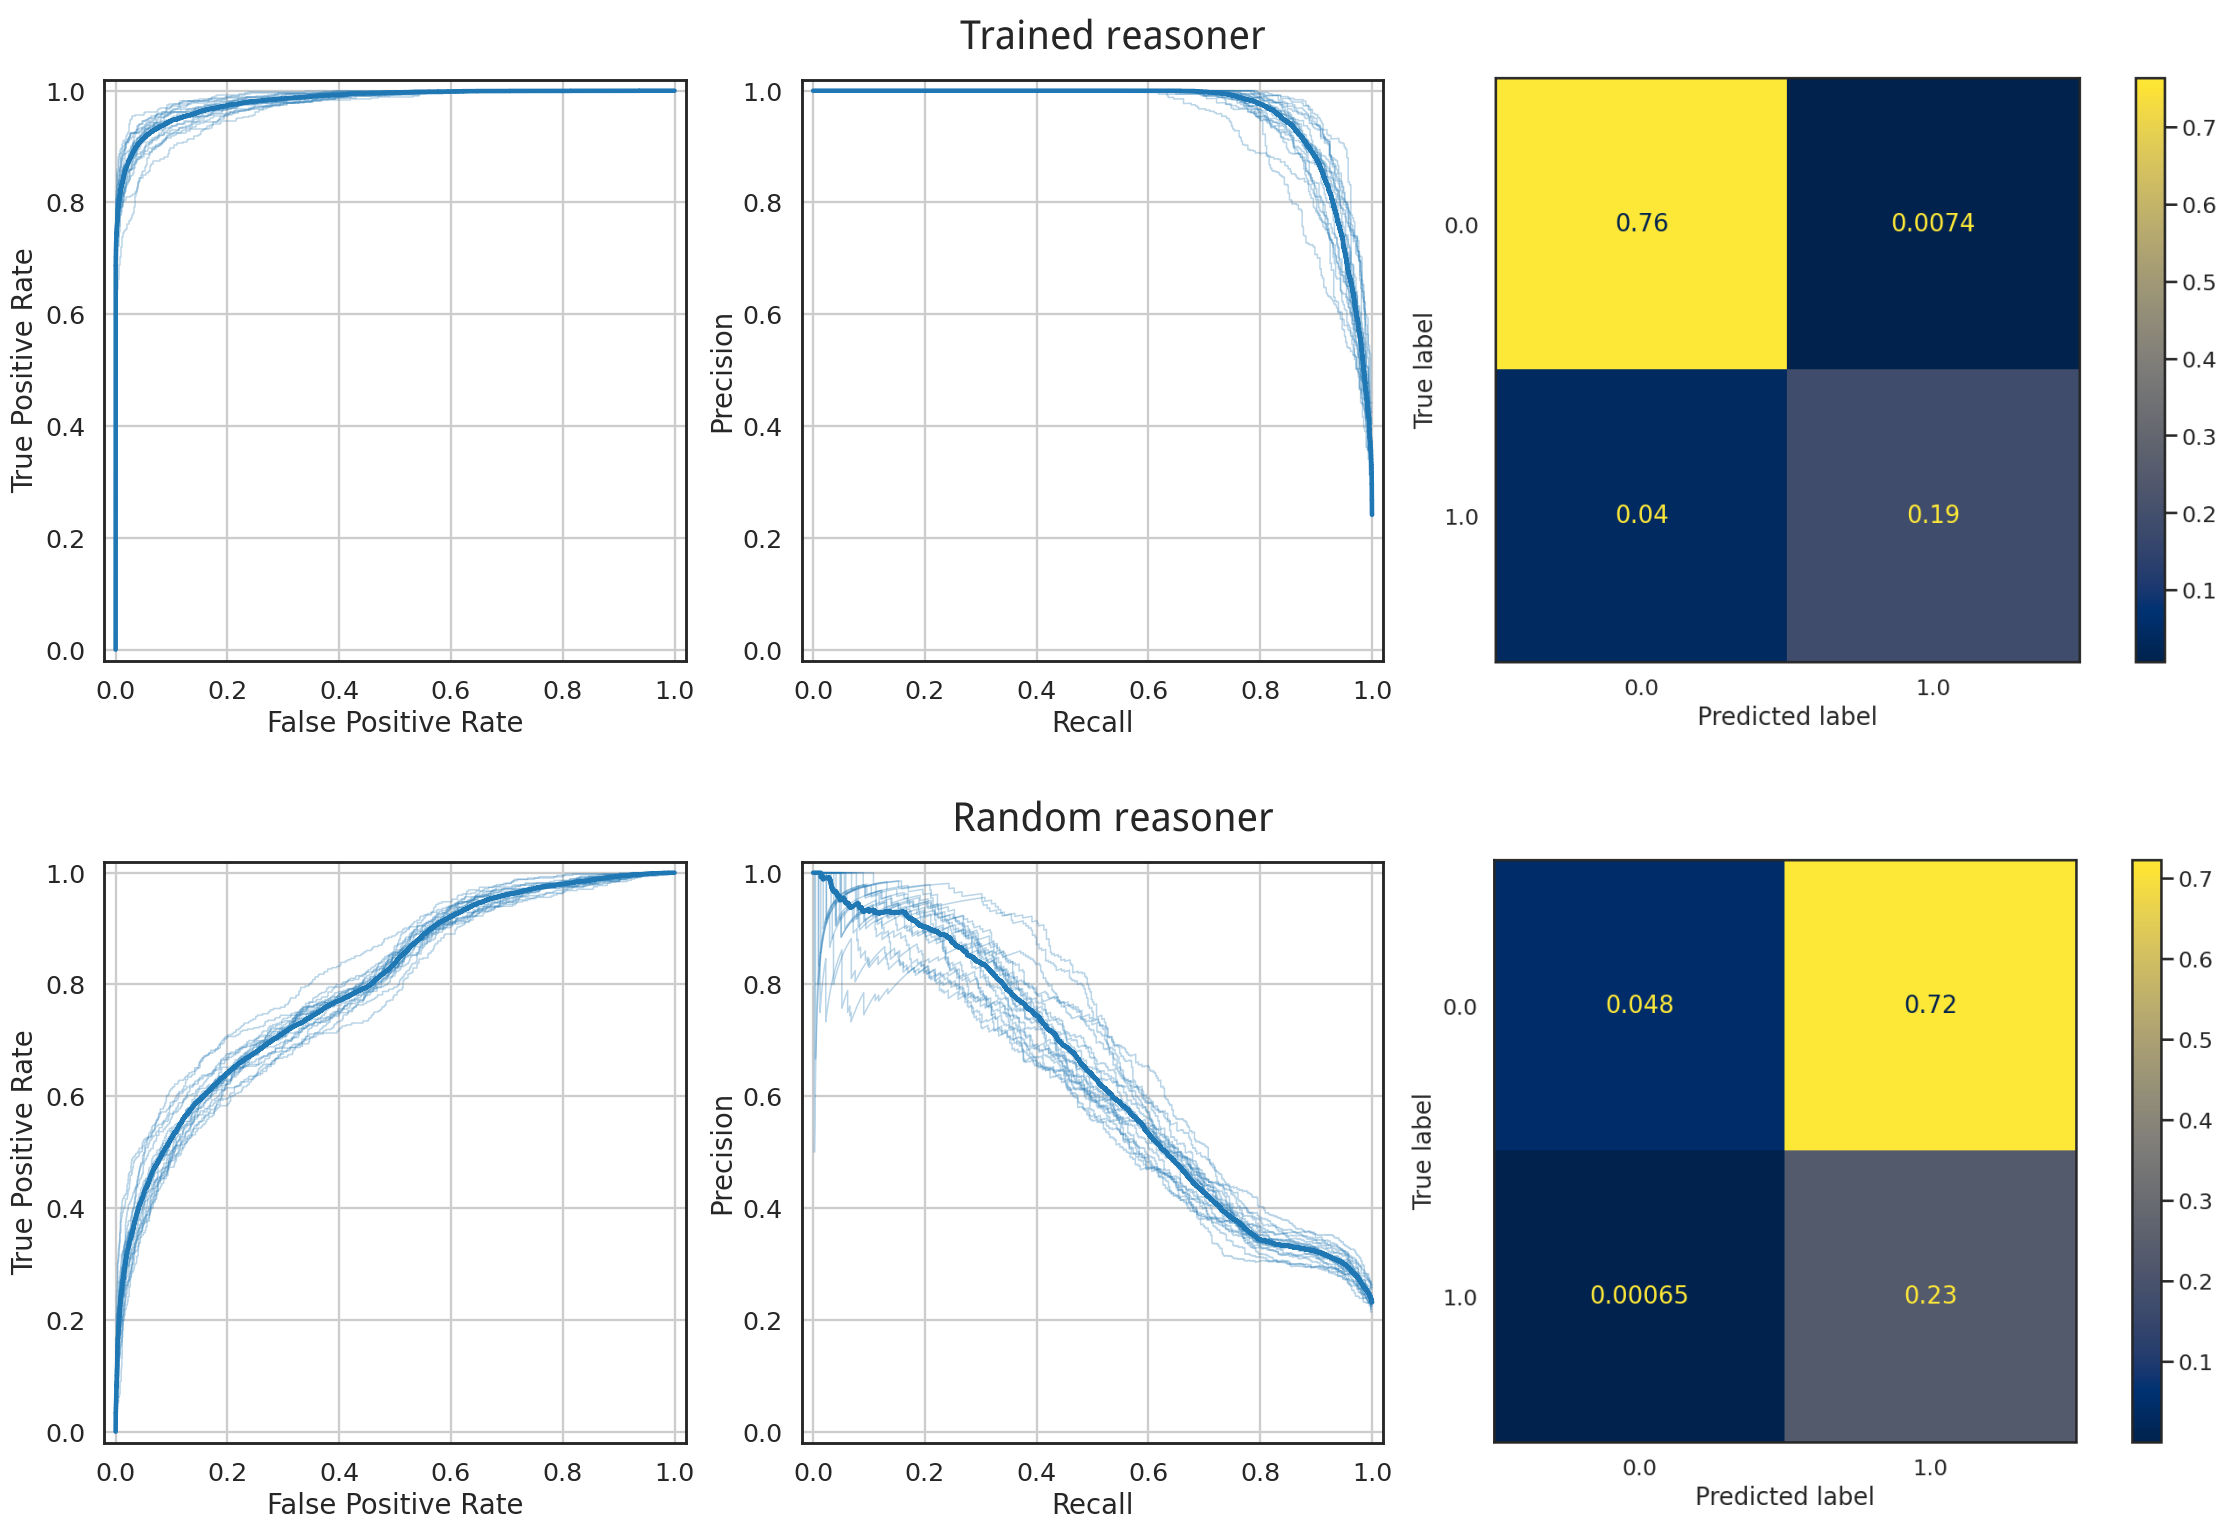
\includegraphics[width=1\linewidth]{figures/ex2-vs.png}
}
\centering
\caption{
ROC curves and confusion matrices for the restricted reasoner.
}
\label{fig:ex2-vs}
\end{figure}


\chapter{Case study -- pizza ontology}
\label{chap:casestudy}

In \autoref{chap:reasoneur} we evaluated our deep neural reasoner in two ways.
Firstly, we showed that our reasoner can learn to accurately classify whether subsumption axioms are entailed by a given KB.
Secondly, we demonstrated that pre-training the reasoner head results in shorter fine-tuning time and greater classification accuracy for unseen KBs, when compared to a randomly initialized reasoner head with no pre-training, which meant that reasoner heads are transferable.
Because the classification metrics were high, we concluded that the learned embeddings encode information that is useful for classifying entailment.
However, since we trained our reasoner on a synthetic data set, the embeddings were not interpretable.

In this chapter we use the pizza ontology\footnote{As a reminder, \emph{ontology} is an OWL term for a knowledge base. Since the pizza ontology is an OWL document, we use the term \emph{ontology} when referring to it. We still use the term \emph{knowledge base}, when referring to KBs in general.}\footnote{The pizza ontology in the RDF/XML format is available at \url{http://owl.cs.manchester.ac.uk/publications/talks-and-tutorials/protg-owl-tutorial/}} from the Manchester University OWL Tutorial~\cite{horridge_practical_2011}
We chose the pizza ontology, because it has a similar number of axioms, concept and role names to the randomly generated KBs we used in experiment 1.
The relatively small number of concept names made it easy to visualize all the learned embeddings, while keeping the visualization readable.
The ontology contains various axioms (equivalence and disjointness axioms, universal and existential restrictions, concept intersection, union, and complement), so we could test all capabilities of our reasoner.
We describe the pizza ontology in detail in~\autoref{sec:pizza-analysis}.

The pizza ontology is described with OWL DL, so to use our reasoner to learn concept embeddings, it was necessary to remove small parts of the ontology because $\SHOIND$ (the underlying logic of OWL DL) is more expressive than $\ALC$.
We describe the process of reading from the RDF/XML format and the steps to transform OWL DL ontologies to $\ALC$ KBs in~\autoref{sec:pizza-preproc}.

After introducing the pizza ontology, we describe experiments 2 and 3.
In experiment 2 we check whether our reasoner is able to learn concept name embeddings of the pizza ontology by learning to classify entailment of subsumption axioms, where both operands are concept names.
In experiment 3 we check whether our reasoner is able to learn complex concept embeddings, by learning to classify entailment of subsumption axioms, where both operands are arbitrary concepts.
We also checked whether using a pre-trained reasoner head would have a beneficial effect on the learned embeddings.
In both experiments, we evaluated the reasoning ability of the trained reasoners according to selected metrics. We also analyze the learned embeddings by visualizing them and subjectively assessing their quality.

\newpage

\section{Summary of the pizza ontology}
\label{sec:pizza-analysis}

To explore the pizza ontology, we used \Protege{} -- the most widely used OWL ontology editor~\cite{musen_protege_2015}. Specifically, we used version 5.5.0 of \Protege, and version 1.6.5 of the \factpp{} reasoner plugin\footnote{Version 1.6.5 of the \factpp{} plugin for \Protege{} 5 is available at \url{https://bitbucket.org/dtsarkov/factplusplus/downloads/uk.ac.manchester.cs.owl.factplusplus-P5.x-v1.6.5.jar}}.

\subsection{Ontology metrics}

\begin{figure}
\centering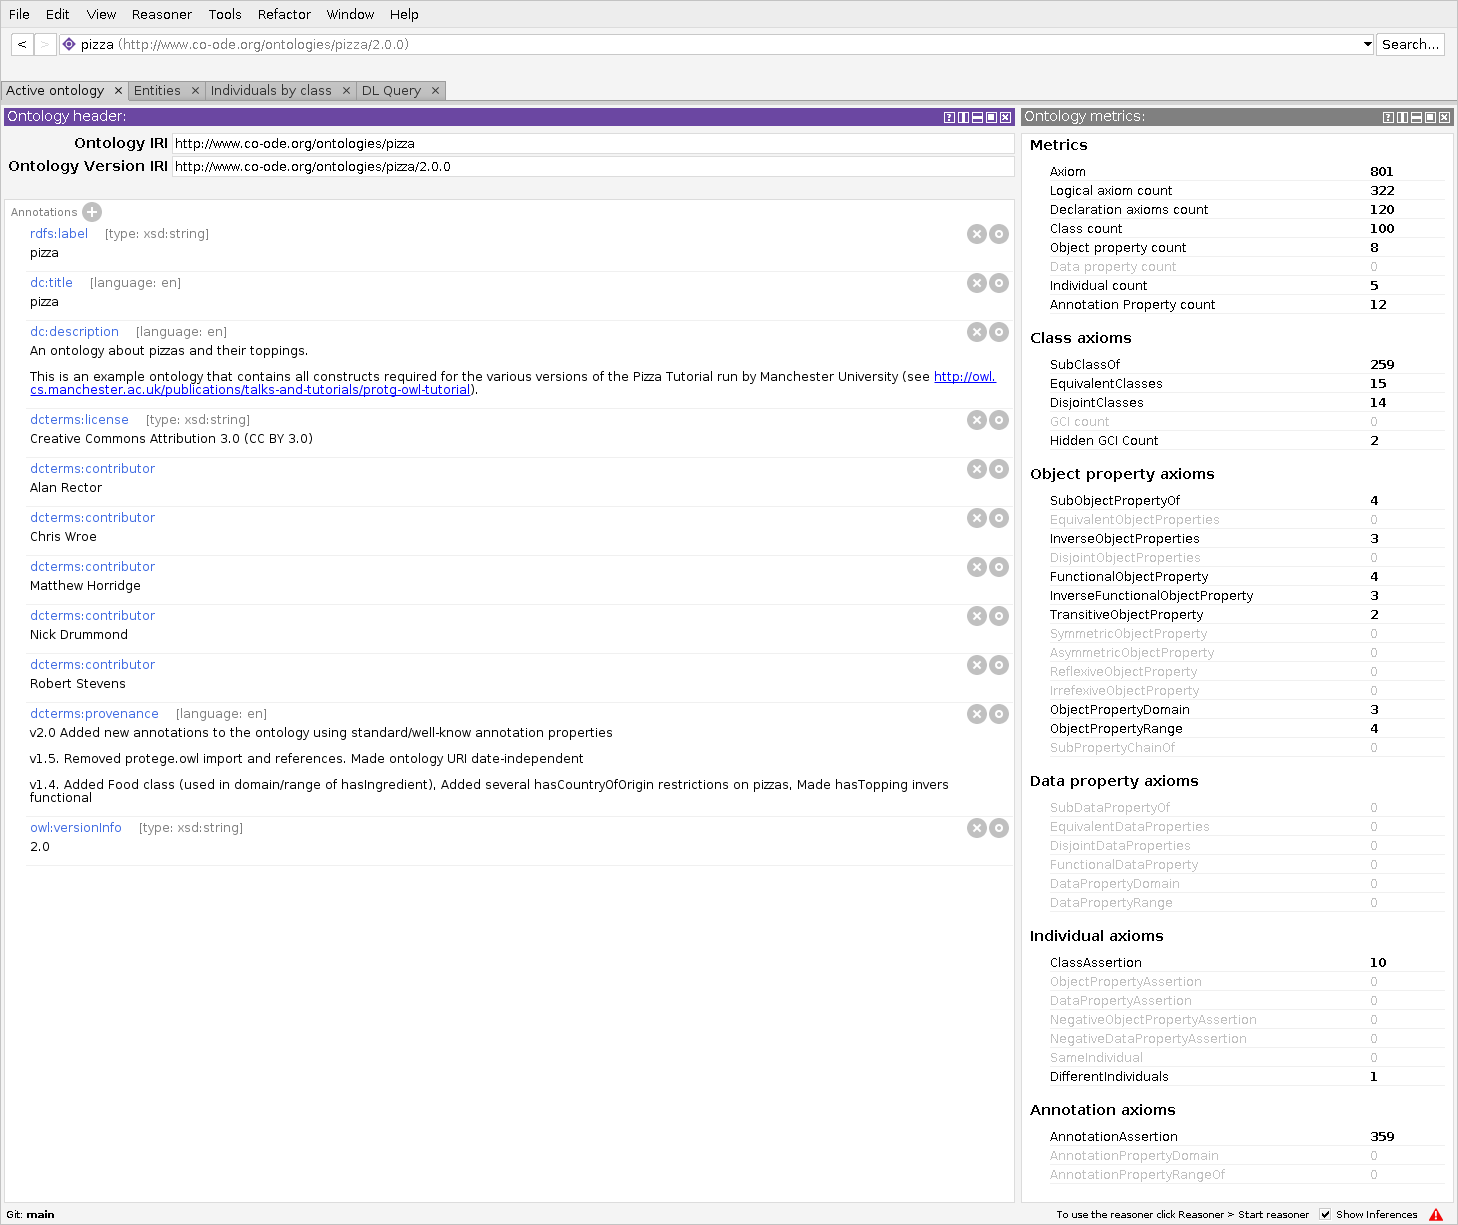
\includegraphics[width=\textwidth]{figures/pizza-summary.png}
\caption{Summary of the pizza ontology in \Protege. Note the ontology metrics on the right}
\label{fig:pizza-summary}
\end{figure}

The summary of the version 2.0 of the pizza ontology is shown in~\autoref{fig:pizza-summary}.
We pay attention to metrics, as they are useful for quickly grasping the contents of an ontology.
According to \Protege{} there are 100 classes and 8 object properties which are equivalent to concept names and role names, respectively.
There are 15 equivalence axioms and 15 class disjointness axioms (in OWL DL, a \tw{Disjoint\-Classes} axiom allows one to specify that given a set of classes, every pair of classes from that set is disjoint).

The pizza ontology contains 23 object property axioms.
Most importantly, properties \tw{has\-Base} and \tw{hasTopping} are subclasses of \tw{has\-Ingredient}.
There are also properties \tw{is\-Base\-Of}, \tw{is\-Topping\-Of} and \tw{is\-Ingredient\-Of}, which are inverses of the aforementioned properties.
The properties \tw{has\-Base}, \tw{has\-Topping}, and \tw{has\-Ingredient} are transitive, and their domain and range are specified.
Another often-used property in the pizza ontology is \tw{has\-Spiciness}, which is used to relate classes to spiciness levels.
Some properties are also defined as functional, or inverse functional, which is irrelevant in our case, since these characteristics cannot be expressed in $\ALC$.

There are 12 annotation properties and 359 annotation assertions.
We use the \tw{rdfs:label} annotation property in English to obtain the name of a class when parsing the ontology in the RDF/XML format.
We also examined the \tw{rdfs:comment} annotations written by the ontology authors, as some of them contained useful explanations.
In particular, the authors explain how \tw{IceCream} and \tw{Cheesy\-Vegetable\-Topping} are purposefully made to be unsatisfiable (equivalent to $\bot$).
The first class is unsatisfiable because \tw{IceCream} was defined as a subclass of $\exists \tw{hasTopping} .
\tw{FruitToping}$, which implies that \tw{IceCream} is a subclass of \tw{Pizza}, since the domain of \tw{hasTopping} was defined to be \tw{Pizza}.
However, \tw{IceCream} was also defined as disjoint with \tw{Pizza}, \tw{PizzaBase} and \tw{PizzaToping}, leading to an inconsistency.
The class \tw{Cheesy\-Vegetable\-Topping} is unsatisfiable because it is defined to be a subclass of both \tw{CheeseTopping} and \tw{VegetableTopping}, but these toppings were defined to be disjoint, so their intersection is equivalent to $\bot$.
Starting the \factpp{} reasoner in \Protege{} confirms that both classes are equivalent to the bottom concept.

There are also 5 individuals, 10 class assertions, and one set of different individuals.
The individuals are \tw{America}, \tw{England}, \tw{France}, \tw{Germany}, and \tw{Italy}, which are instances of the class \tw{Country}.
Similarly to disjointness axioms, OWL DL allows one to specify that none of the individuals in a given set are the same with an \tw{Different\-Individuals} axiom.
All individuals in the pizza ontology are defined as different.
The \tw{American} and \tw{AmericanHot} pizzas are defined as subclasses of value restriction \tw{has\-Country\-Of\-Origin value America}.
Similarly, the object property \tw{has\-Country\-Of\-Origin} is used to relate the individual \tw{Italy} with \tw{Napoletana}, \tw{Veneziana}, \tw{Mozzarella\-Topping}, and \tw{Real\-Italian\-Pizza}.

\subsection{Class hierarchy}

\begin{figure}
\centering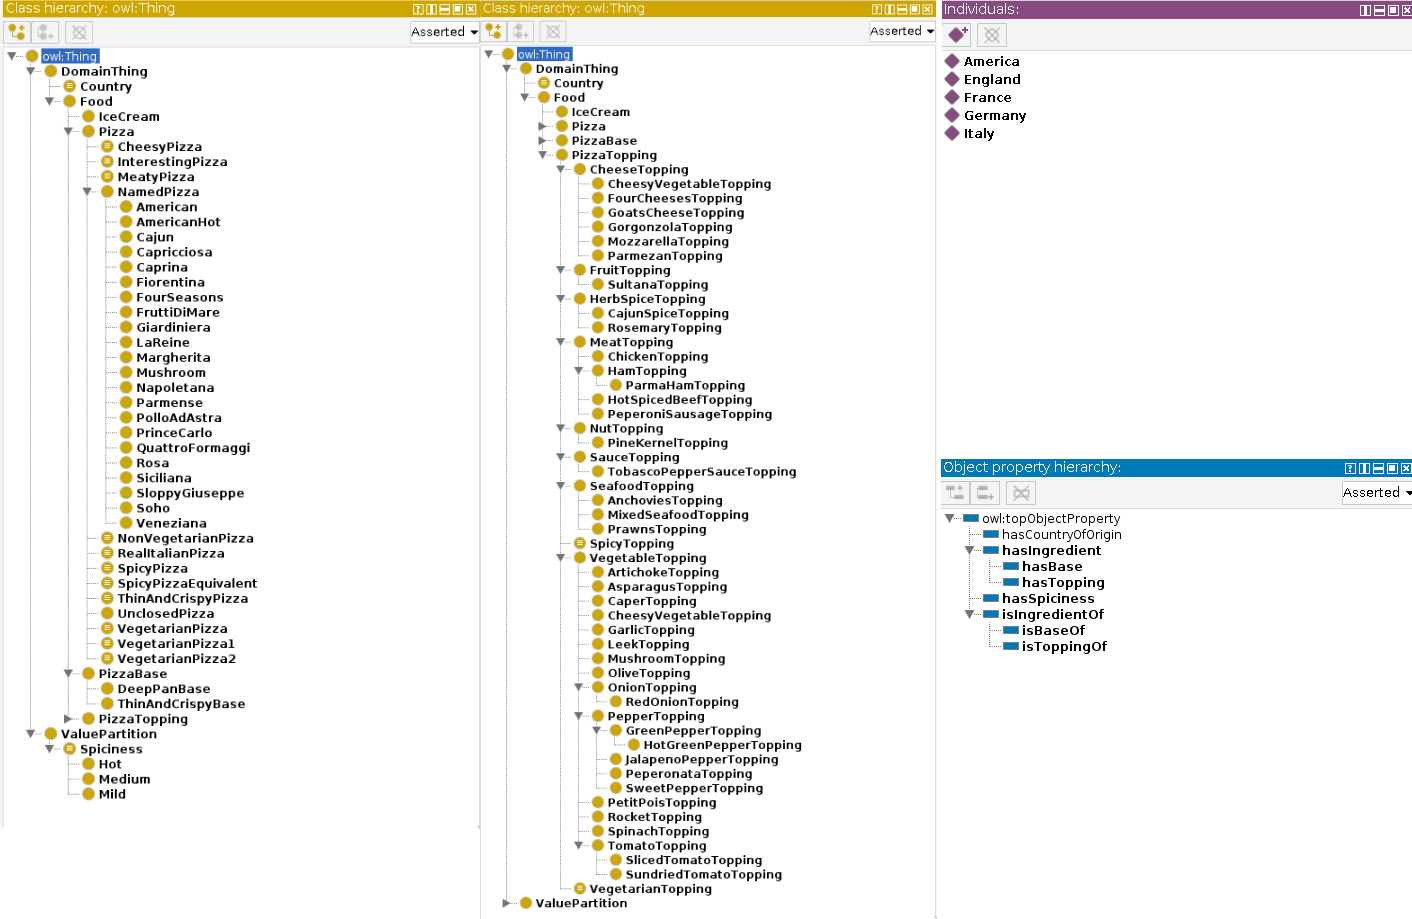
\includegraphics[width=\textwidth]{figures/pizza-hierarchy.png}
\caption{Class hierarchy, role hierarchy, and individuals in the pizza ontology, shown in \Protege{}. The entire vocabulary of the ontology is visible.}
\label{fig:pizza-hierarchy}
\end{figure}

We also familiarized ourselves with the class hierarchy of the ontology (shown in~\autoref{fig:pizza-hierarchy}).
All classes are of course subclasses of the top concept (\tw{Thing} in OWL nomenclature), but the only direct subclasses of $\top$ are \tw{Domain\-Thing} and \tw{Value\-Partition}, which are disjoint.

\tw{Spiciness} is a direct subclass of \tw{Value\-Partition}, and is defined as equivalent to the union of three disjoint classes: \tw{Hot}, \tw{Medium}, and \tw{Mild}, which effectively partitions \tw{Spiciness} into three non-overlapping subsets.

\tw{Country} and \tw{Food} are the only direct subclasses \tw{Domain\-Thing} class.
\tw{Country} is defined as the set of 5 countries (individuals) in this ontology.
\tw{Food} is divided into \tw{IceCream}, \tw{Pizza}, \tw{PizzaBase} and \tw{PizzaTopping}.
Not including \tw{Domain\-Thing} and \tw{Food}, the \tw{Pizza} and \tw{PizzaTopping} classes contain the most subclasses in the pizza ontology, with slightly more pizza toppings than pizzas.

\tw{NamedPizza} is a subclass of \tw{Pizza} and has 23 real-world pizzas as subclasses.
Other subclasses of \tw{Pizza} are defined with equivalence axioms, so their subclasses are inferred by a reasoner.
Notably, there are \tw{Vegetarian\-Pizza}, \tw{Vegetarian\-Pizza1} and \tw{Vegetarian\-Pizza2} classes, which define vegetarian pizzas differently.
\tw{Vegetarian\-Pizza1} and \tw{Vegetarian\-Pizza2} are actually equivalent, and they are inferred to be subclasses of \tw{Vegetarian\-Pizza}, but they are not equivalent to it.
Another interesting pizza is \tw{UnclosedPizza}, which is defined as a subclass of $\exists \tw{hasTopping} . \tw{Mozzarella\-Topping}$.
A reasoner cannot actually infer that \tw{UnclosedPizza} is a subclass of \tw{VegetarianPizza} or \tw{Non\-Vegetarian\-Pizza}, because due to the open-world assumption (OWA), it may have other, possibly non-vegetarian toppings.
If \tw{UnclosedPizza} would be defined as $\forall \tw{hasTopping}. \tw{Mozzarella\-Topping}$, then it could be classified as a vegetarian pizza. In total, there are 35 subclasses of \tw{Pizza}, 14 subclasses of \tw{Vegetarian\-Pizza}, and 15 subclasses of \tw{Non\-Vegetarian\-Pizza}.

The topping hierarchy is relatively simple, as it consists of cheese, fruit, herb/spice, meat, nut, sauce, seafood, and vegetable toppings.
The only toppings defined using equivalence axioms are \tw{VegetarianTopping} and \tw{SpicyTopping}.
Vegetarian toppings are defined as a union of cheese, fruit, herb/spice, nut, sauce, and vegetable toppings.
Spicy toppings are defined as toppings that are a subclass of $\exists \tw{hasSpiciness} . \tw{Hot}$.
In total, there are 51 subclasses of \tw{PizzaTopping}, 39 subclasses of \tw{VegetarianTopping}, 7 subclassess of \tw{SpicyTopping}.

In addition to \tw{PizzaBase}, there are only two disjoint pizza bases: \tw{DeepPanBase} and \tw{Thin\-And\-Crispy\-Base}.
These are rarely used, as \tw{Thin\-And\-Crispy\-Base} is only used to define \tw{Real\-Italian\-Pizza} and \tw{Thin\-And\-Crispy\-Pizza}, and \tw{Deep\-Pan\-Base} is not used in any pizza-related axioms at all.


\subsection{Ontology processing}
\label{sec:pizza-preproc}

The pizza ontology is available online in RDF/XML format.
Although we could easily view the ontology in \Protege{}, using our reasoner to learn concept embeddings requires that the ontology is stored in a format closer to the syntax of $\ALC$.
As we mentioned, it is also necessary to remove parts of the ontology to make it compatible with our neural reasoner, because the pizza ontology is described with $\SHOIND$, which is the underlying logic of OWL DL, and is more expressive than $\ALC$.

%\subsection{Parsing}

To parse the pizza ontology, we first use the ROBOT command-line tool to convert it from RDF/XML to the OWL functional-style syntax.
After the conversion, we use our parser to load the ontology into our in-memory KB representation.
We described our parser and the KB representation in~\autoref{sec:technologies}.

% no thanks to owlready2 :)

%\subsection{Pre-processing}

We do the following pre-processing steps to make OWL ontologies compatible with our reasoner.
Pre-processing is done automatically after parsing the ontology file, so one does not need to edit the ontology manually.

\begin{itemize}
\item As the string value of concept names, we use the value of the \tw{rdfs:label} annotation property for the English language.
\item We ignore object property axioms, since role axioms are not expressible in $\ALC$ (including role hierarchies, inverse roles, transitive roles, and (inverse) functional roles).
\item We ignore axioms with number or value restrictions, since they are not expressible in $\ALC$ with KBs where ABox is empty.
\item We ignore individuals and ABox axioms, since our reasoner does not support ABox reasoning.
\item Since our reasoner does not directly support equivalence axioms $C \equiv D$, we split such axioms into two subsumption axioms $C \sub D$ and $D \sub C$, as equivalence can be reduced to subsumption~\cite{baader_basic_2003}.
\item Our reasoner also does not directly support disjointness axioms, so given a disjointness axiom $\tw{DisjointClasses}(A_1, A_2, \ldots, A_n)$ in the OWL functional-style syntax, we generate axioms $A_i \dland A_j \sub \bot$, for each possible pair of concept names $(A_i, A_j)$ from the set of disjoint concepts, where $A_i \neq A_j$.
\item We remove roles that do not appear in any TBox axiom kept after pre-processing. This is done because of a limitation in \factpp{}, which makes it raise an exception, when constructing a concept with an unused role name.
\end{itemize}

%\subsection{Consequences for the pizza ontology}

After processing the pizza ontology, \tw{Interesting\-Pizza} is equivalent to the top concept, because the axiom defining it as a pizza with at least 3 toppings contained a number restriction, so it was removed.
The equivalence axiom that defines \tw{Real\-Italian\-Pizza} as a pizza with Italy as its country of origin was removed because it contained a value restriction.
Since \tw{Real\-Italian\-Pizza} was also defined as a subclass of $\exists \tw{hasBase} .\tw{Thin\-And\-Crispy\-Base}$, any pizza with a thin and crispy base is inferred to be a subclass of \tw{Real\-Italian\-Pizza}.
Value restrictions for \tw{American}, \tw{AmericanHot}, \tw{Napoletana}, \tw{Veneziana}, and \tw{MozzarellaTopping} were removed, but that did not have a significant effect on reasoning.

After loading the pizza ontology, we observed that only 99 classes are actually defined in the ontology, instead of 100 reported by \Protege{}.
This can be easily confirmed by saving the pizza ontology with \Protege{} in the OWL functional-style syntax format and counting the number of \tw{Declaration(Class(...))} expressions in the resulting file.
We do not know what in the pizza ontology is counted as the extra class by \Protege{}, but in this chapter we assume that the number of concept names is $|N_c| = 99$, which is consistent with the source file of the pizza ontology and our ontology processing code.

We used \factpp{} to classify the ontology after processing, and visualized the result as a heat map (shown in~\autoref{fig:pizza-heatmap}).
 
\begin{figure}
\makebox[\textwidth][c]{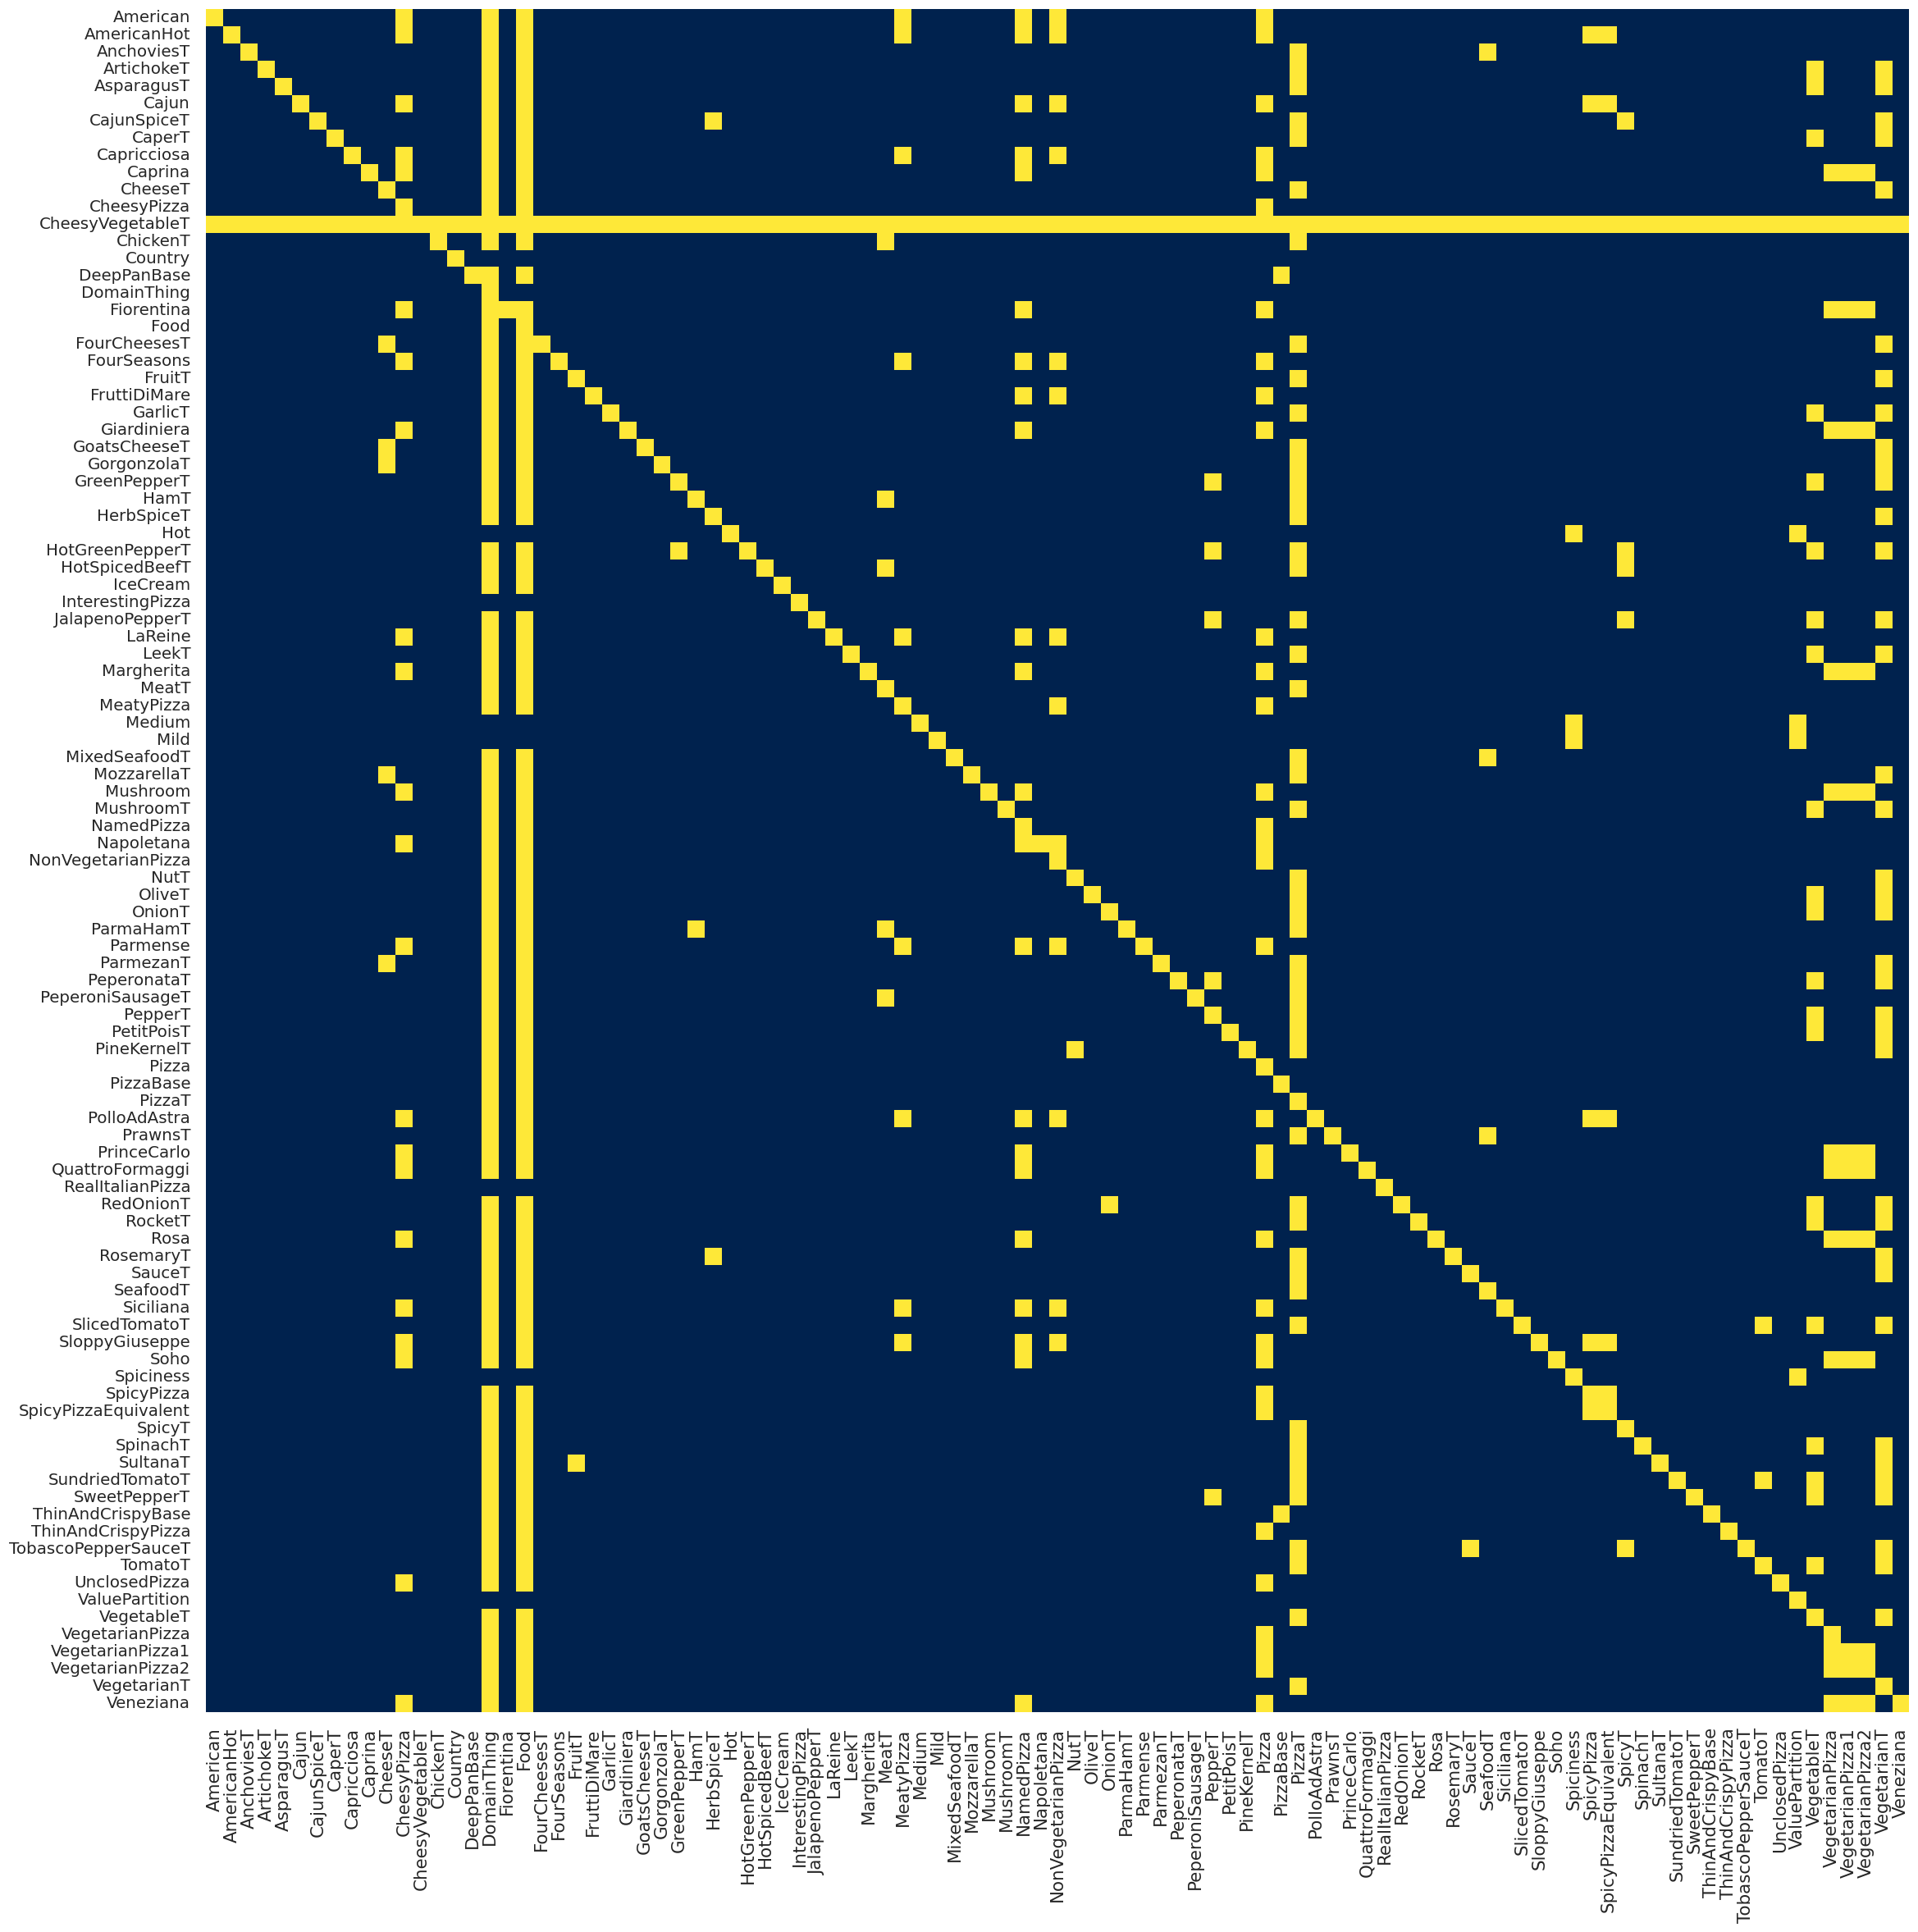
\includegraphics[width=1.2\textwidth]{figures/pizza-heatmap.png}}
\caption{
Results of ontology classification with \factpp{}.
Each heat map cell shows the result of query $\KB \models A_i \sub A_j$, where $i$ is the heat map row, $j$ is the heat map column and $A_k$ is the k-th concept name in the pizza ontology in lexicographical order ($A_1$ being \tw{American} and $A_{99}$ being \tw{Veneziana}).
We replaced the word ``Topping'' in concept names with ``T'' to save space.
A concept that is subsumed by every concept (a concept equivalent to $\bot$) is shown as a yellow horizontal line, and a concept that subsumes every concept (a concept equivalent to $\top$) would be shown as a yellow vertical line.
}
\label{fig:pizza-heatmap}
\end{figure}

\section{Experiment 2 -- Pizza taxonomy}

After parsing and processing the pizza ontology, it can be used to test our reasoner. In this experiment, we show that given a simple data set, our reasoner can easily learn good embeddings for concept names.

\subsection{Data set generator}

The data set for this experiment is very simple.
It consists of all possible queries $\KB \models C \sub D$, where $C$ and $D$ are concept names or $\top$ or $\bot$.
Since the pizza ontology contains 99 classes, in addition to $\top$ and $\bot$, the number of queries in this simple data set is equal to $(|N_C| + 2)^2 = (99 + 2)^2 = 10201$.
The answers to all queries were obtained using the \factpp{} reasoner.
We recognize that for any concept $C$, queries $C \sub C$, $C \sub \top$, and $\bot \sub C$ can be trivially answered.
However, because we are training the reasoner for the pizza ontology from scratch, we want it to learn to correctly classify those queries too.

The resulting data set is not balanced, as only about 868 queries ($\approx 8.5\%$) are assigned to class $1$, and the remaining 9333 queries ($\approx 91.5\%$) are assigned to class $0$.
We do not perform under-sampling or oversampling, as even with this unbalanced data set, our reasoner learns embeddings that allow it to classify all entailment queries almost perfectly.

\subsection{Model and training procedure}

In this experiment, we train a reasoner using the restricted architecture.
We train the reasoner from scratch -- that is, we randomly initialize the reasoner head and embedding layer.
We pick a small embedding dimension $N_e = 10$, which is significantly smaller than the number of classes in the pizza ontology and forces the reasoner to share embedding dimensions between concepts.
We set the size of the hidden layer of the entailment checking neural network $\nn_\sub$ to 16, which is the same as in experiment 1.

With the aforementioned hyperparameters, the reasoner head has 1963 learnable parameters in total ($(2N_e + N_e^2 + 1) \cdot 16 + (16 + 1) \cdot 1 = 1953$ parameters in $\nn_\sub$, and $N_e$ parameters for the bottom concept), and the embedding layers have 1000 parameters ($N_e$ parameters per concept name, and $N_e$ for the top concept), which is 2953 parameters in total.
We did not include parameters of role embeddings $\nn_{\KB,R_i}$, and the intersection and negation constructor networks $\nn_\dland$ and $\nn_\lnot$, as the data set in this experiment does not use them.

We do not split the data set, since we want the learned concept embeddings to fit the data set as well as possible.
We train the reasoner and embeddings for 30 epochs.
After each training epoch, we calculated classification metrics for the entire data set.
We use the AdamW optimizer with learning rate set to the same value for both reasoner head and embedding layer optimizers $\eta_c = \eta_e = 0.002$.

\subsection{Evaluation of reasoning ability}

After training for 30 epochs, the reasoner achieves perfect classification metrics.
In total, at the threshold of 0.5, the trained reasoner made 0 mistakes.
Because the error rate is 0, we do not show the heat map of the predicted probabilities, as it looked exactly the same as the heat map in~\autoref{fig:pizza-heatmap}.

Of course, we realize that the $\nn_\sub$ network in the reasoner head simply memorized answers to the queries from the data set.
Nevertheless, it was useful to verify that the reasoner can at least find embeddings that are helpful in learning the entailment relation for a simple taxonomy.


\subsection{Embedding analysis}
\label{sec:pizzaviz}

In addition to evaluating the reasoning ability of our reasoner, which showed that it can successfully learn to classify entailment of subsumption axioms in a ``real-world'' KB, we visualize the learned embeddings.

A 2D visualization that tries to preserve the distances between concepts in the high-dimensional embedding space enables visual assessment of the quality of the learned embeddings.
We think that if semantically similar concepts are placed closer to each other than to dissimilar concepts, then the learned embeddings capture the semantics of a given KB.

\subsubsection{Dimensionality reduction}

Because we chose 10 as the size of concept embeddings, first we needed to reduce the dimensionality of the embeddings.
We used Uniform Manifold Approximation and Projection for Dimension Reduction (UMAP), because it is a nonlinear dimensionality reduction algorithm with interpretable hyperparameters and high performance~\cite{mcinnes_umap_2020}.
We used the Python implementation by the authors of UMAP and other open source contributors\footnote{Source code for the Python UMAP implementation is available at \url{https://github.com/lmcinnes/umap}}.

According to UMAP's documentation, the two main hyperparameters are \tw{n\_neighbors} and \tw{min\_dist}.
The first one specifies the number of neighbors to consider during the initial construction of the high-dimensional graph.
Low values of \tw{n\_neighbors} emphasize the local structure of the data, and high values emphasize the global structure of the data.
The second hyperparameter specifies the minimum distance between points in the low-dimensional space.
Low values of \tw{min\_dist} will result in visualizations where the clusters are tightly packed and high values will spread out the data points.

For our purposes, we wanted to emphasize the global structure of the learned embeddings, so we set \tw{n\_neighbors} at a very high value of 50 (considering that we have 101 points in total).
To choose the value of \tw{min\_dist} we began at 0.99 and decreased the value until the visualization became readable and clusters started to separate.
In the end, we set the value of \tw{min\_dist} at 0.01.

\subsubsection{Coloring scheme}

If we visualized all concept embeddings as points sharing the same shape and color, our visualization would not be readable, and it would be hard to judge, whether semantically similar concepts form clusters.
To create an effective visualization of the learned embeddings, we created a coloring scheme for concepts in the pizza ontology that tries to make the most important attributes of concepts immediately recognizable.
The following description specifies how we use different shapes, sizes, and colors of markers:

\begin{itemize}
    \item By default concepts are square and gray
    \item Top concept, bottom concept and concept expression are cyan
    \item Toppings are shaped like diamonds, and pizzas are round
    \item Vegetarian pizzas and toppings are light green (except vegetable toppings, which are dark green)
    \item Seafood toppings are pink
    \item Non-vegetarian pizzas and meat toppings are dark red
    \item Cheesy pizzas, and cheese toppings are respectively marked with a yellow disk or yellow diamond inside
    \item Pepper toppings are marked with an orange diamond inside
    \item Spicy things are marked with a red ``x'' inside
    \item Spiciness levels are light red 
\end{itemize}

\subsubsection{Visual assessment}

\begin{figure}
\centering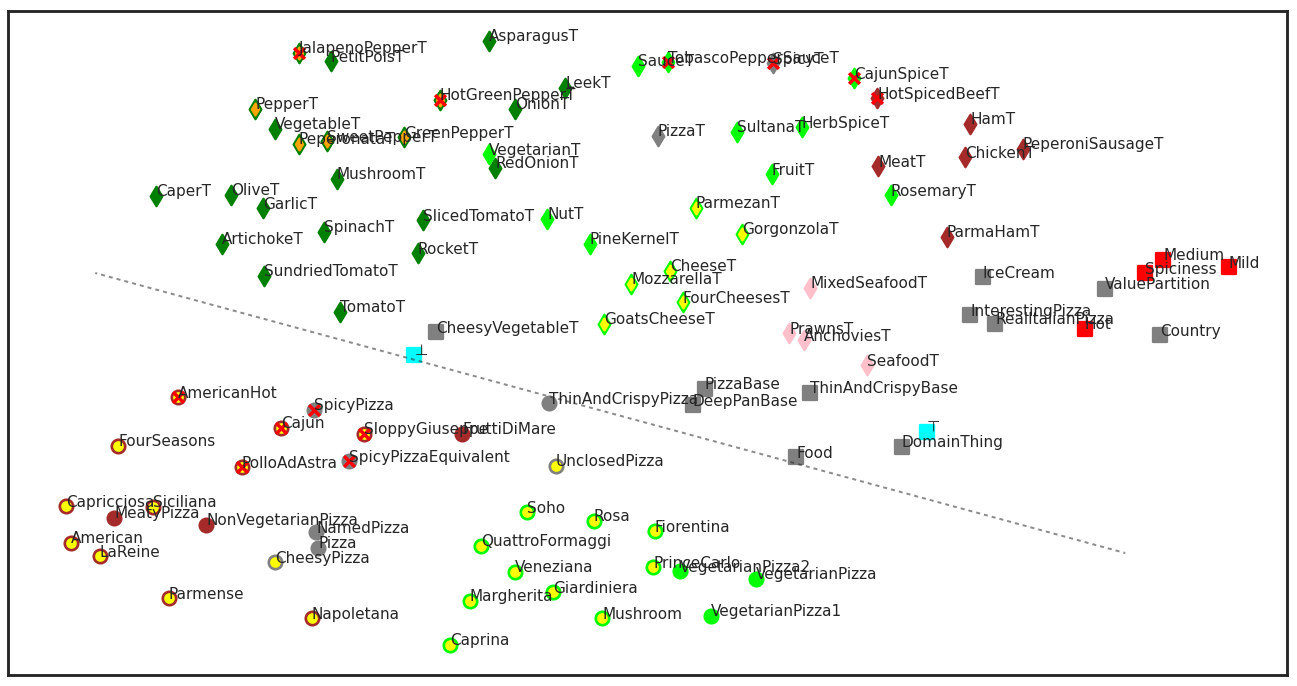
\includegraphics[width=\textwidth]{figures/ex3-emb.png}
\caption{UMAP visualization of the learned concept embeddings. The shapes and colors of the point markers are decided according to the scheme described in~\autoref{sec:pizzaviz}. We replaced ``Topping'' in concept names with ``T'' to improve readability. The dashed line separating pizzas from other concept names was added for emphasis.}
\label{fig:ex3-emb}
\end{figure}

The UMAP visualization of the concept embeddings is shown in~\autoref{fig:ex3-emb}.
As expected, the unsatisfiable \tw{Cheesy\-Vegetable\-Topping} is close to $\bot$, and the general \tw{Domain\-Thing} concept is close to $\top$.
Spiciness and pizza bases form their own clusters.
Pizzas and toppings are separated, with vegetarian pizzas forming one cluster, and non-vegetarian pizzas forming another cluster together with spicy pizzas.
All spicy pizzas in the pizza ontology are non-vegetarian, so it is understandable that \tw{Spicy\-Pizza} and \tw{Spicy\-Pizza\-Equivalent} are close to non-vegetarian pizzas.

Meat toppings are close to each other and relatively close to seafood toppings, which is good.
Cheesy toppings, vegetable toppings, spicy toppings, and pepper toppings are also close to related concepts.
\tw{Cajun\-Spice\-Topping} is close to \tw{Hot\-Spiced\-Beef}, which is understandable, because they are both spicy toppings.
\tw{Meat\-Topping} and \tw{Rosemary\-Topping} are also close to each other, which is unexpected. 

Overall, based on the visualization, we think the embeddings capture the semantics well, given the simple data set.


\section{Experiment 3 -- Full data set}

The previous experiment showed that our reasoner can learn good concept embeddings for simple taxonomies, so the next step is to test whether it can learn good embeddings for arbitrary concepts.
In this experiment we do that by training the neural reasoner to classify entailment, given randomly generated queries about the pizza ontology as the data set.
We repeat this experiment three times.
In the first run, we let the reasoner learn without any pre-training.
In the second run, we initialize the reasoner head with weights of the restricted reasoner, that we trained in experiment 1, then freeze it, and only allow the embedding layer to learn.
In the third run, we randomly initialize the reasoner head, and also freeze it to only allow the embedding layer to learn KB-specific embedding.

\subsection{Training data set}

The data set for this experiment consists of $30\ 000$ unique random queries that we generate using the algorithm described in~\autoref{sec:random_axiom}.
We set the maximum axiom depth to 4, and the probability of concept names to $p_A = 0.95$.
The answer to each query is obtained using \factpp{}.
Similarly to the last experiment, we do not split the data set because we want the learned embeddings to fit the data set as well as possible.
The data set is slightly imbalanced, with 36.97\% of queries belonging to class $y = 1$, and the rest to class $y = 0$, although the class imbalance did not significantly affect classification.

\subsection{Training procedure}

As mentioned, we repeat learning three times, which results in three reasoners:

\begin{itemize}
    \item \emph{Unfrozen reasoner head} -- Both the reasoner head and KB-specific embedding layers were trained.
    \item \emph{Frozen pre-trained reasoner head} -- Only KB-specific embedding layers were trained. The reasoner head head was initialized with the weights of the restricted reasoner, that we obtained in experiment 1.
    \item \emph{Frozen random reasoner head} -- Only KB-specific embeddings layers were trained. The reasoner head was initialized randomly.
\end{itemize}

Each reasoner head has 3283 learnable parameters in total ($(2N_e + N_e^2 + 1) \cdot 16 + (16 + 1) \cdot 1 = 1953$ parameters for $\nn_\sub$, $(2N_e + N_e^2 + 1) \cdot N_e = 1210$ parameters for the concept intersection constructor $\nn_\dland$, $(N_e + 1) \cdot N_e = 110$ parameters for the concept complement constructor $\nn_\lnot$, and $N_e$ parameters for the bottom concept), and the embeddings have 1330 parameters ($N_e$ parameters per concept name, $N_e$ for the top concept, and $(N_e + 1) \cdot N_e$ per role), which is 4613 parameters in total.

In every run of the experiment we trained the model for 30 epochs, with learning rate set to $\eta_c = \eta_e = 0.002$ both for the optimizer of the reasoner head and the embedding layers.
Similarly to the previous experiments, we use the AdamW optimizer, and train the reasoners with batch size of 32. 
Because we initialize the frozen pre-trained reasoner head with weights of the restricted reasoner head, that we trained in experiment 1, the embedding dimension $N_e$ and the layers of the neural network $\nn_\sub$ needed to be exactly the same as in that experiment.
Thus, for all reasoners in this experiment we set $N_e = 10$ and defined $\nn_\sub$ to be a neural network with one hidden layer with 16 neurons and ELU activation function.
The embedding dimension is adequate, since the pizza ontology has a similar number of concepts to the ontologies in the synthetic data set, that we used in experiment 1.

We expected the reasoner with the unfrozen head to achieve best metric values and learn the best embeddings out of the three reasoners in the embedding analysis, because no weights are frozen, which means that the reasoner with the unfrozen head can fit to the data set more than the reasoners with frozen heads.
The only obstacle to learning good embeddings for the reasoner with unfrozen head are the randomly generated queries, that may not contain useful entailments for the pizza ontology, although the other two reasoners learn with the same data set, so the comparison is at least fair.

Based on the results of experiment 1, we expected the reasoner with transfer to achieve higher classification metrics than the reasoner with randomly initialized frozen head.
In experiment 1, the trained reasoner head was better at classifying queries for the unseen KBs from the test data set, than the randomly initialized reasoner head, so we expected the same to be true for the pizza ontology.


\subsection{Evaluation of reasoning ability}

\begin{table}
\caption{Classification metrics for reasoners in experiment~3 after training for 30 epochs.}
\label{tab:transfer-test-pizza}
\begin{adjustwidth}{-2cm}{-2cm}
\centering
\begin{tabular}{lcccccc}
\toprule
Model                            & AUC ROC & F1     & Accuracy & Precision & Recall & Training time \\
\midrule
Unfrozen reasoner head           & 0.9997 & 0.9906 & 0.9931 & 0.9915 & 0.9897 & 349.83s \\
Frozen pre-trained reasoner head & 0.9868 & 0.9472 & 0.9612 & 0.9566 & 0.9379 & 290.14s \\
Frozen random reasoner head      & 0.7816 & 0.7372 & 0.7568 & 0.6128 & 0.9249 & 287.21s \\
\bottomrule
\end{tabular}
\end{adjustwidth}
\end{table}

The classification metrics of the three reasoners are shown in~\autoref{tab:transfer-test-pizza}.
The expected ontology classification heat map and heat maps for the three reasoners are shown in~\autoref{fig:ex4-heatmap}.
The ROC curves, PR curves, and confusion matrices for each reasoner are shown in~\autoref{fig:ex4-vs}.

As expected, the unfrozen reasoner achieves strictly better classification performance than the reasoners with frozen heads, as the values of all metrics are higher than for other reasoners.
In particular, the unfrozen reasoner achieves near perfect AUC ROC and accuracy scores, and very good F1-score, precision and recall scores.
The ROC and PR curves for the unfrozen reasoner are nearly perfect, which we also expected.
The ontology classification heat map is close to the expected one, but the unfrozen reasoner has trouble classifying trivial axioms $C \sub D$, where $C = D$.
Perhaps reasoners would classify trivial axioms better if $\nn_\sub$ had more hidden layers, or the layers were wider.
We discuss this and other opportunities for improvement in~\autoref{sec:further-work}.

The reasoner with the frozen pre-trained head is the second-best reasoner after the unfrozen reasoner.
It achieves very high AUC ROC, F1-score, accuracy, and precision, although recall could be improved. 
The ROC and PR curves for the frozen pre-trained reasoner head also indicate a good fit to the data set.
The ontology classification heat map for this reasoner sheds some light on the limitations of knowledge transfer in this learning context. 
Because we chose a small embedding dimension $N_e = 10$, relative to the number of concepts $|N_C| = 99$, if the reasoner head is frozen, then the rather sparse ontology classification map cannot be learned perfectly.
For the unfrozen reasoner, learning the ontology classification was easy, because the weights of the deep neural network $\nn_\sub$ could be adjusted, which compensated for the small embedding dimension. 
For the reasoner with a frozen head, the only option is to adjust the concept embedding vectors and role constructor networks $\nn_{\KB,R_i}$.
Given the high classification accuracy and a good ontology classification heat map, we think that the restricted reasoner in experiment~1 learned good concept complement and intersection constructors $\nn_\lnot$ and $\nn_\dland$.
However, those constructors are limited, so we interpret the recurring vertical and horizontal lines on the heat map, as attempts to place a concept name embedding closer to the embedding of $\top$ and $\bot$, respectively.
This may be done because some concepts like \tw{Food} are general, so for classification it may be useful to just equate it with $\top$, if a better embedding cannot be learned.
We also suspect that for reasoners with frozen heads, the ontology classification may be easier to learn in ontologies that have a larger number of role names $|N_R|$, than for simple taxonomies, because the embedding layer has more parameters, allowing the reasoner to achieve a better fit to the training data.

The reasoner with the randomly initialized frozen head was the worst of the three reasoners, although it is better than a random guesser, with AUC ROC of around 0.78.
This reasoner has very high recall, but relatively low precision.
Looking at the confusion matrix, one can see that the random head has a much higher number of false positives, which explains the low precision score.
The number of false negatives is similar to frozen reasoner head (trained), so the main difference between them is that the randomly initialized reasoner head has much lower precision.
By looking at the ontology classification heat map we can see part of the reason for the low precision -- it is composed almost entirely of uniform vertical and horizontal lines. 
This shows that most named concepts are classified similarly to the top and bottom concept.

For all reasoners there are a bit more false negatives than false positives, which we attribute to the slight class imbalance in the training data set.
For the randomly initialized reasoner, we do not attribute the high number of false positives to the class imbalance, as class $y = 1$ is the minority one, which would typically result in a high number of false negatives instead.
However, the number of false negatives of frozen random reasoner head is similar to the number of false negatives of frozen reasoner head (trained).
We do not think that addressing the class imbalance would significantly improve classification results, as those are already very good for reasoners other than the one with the random head.

\begin{figure}
\makebox[\textwidth][c]{
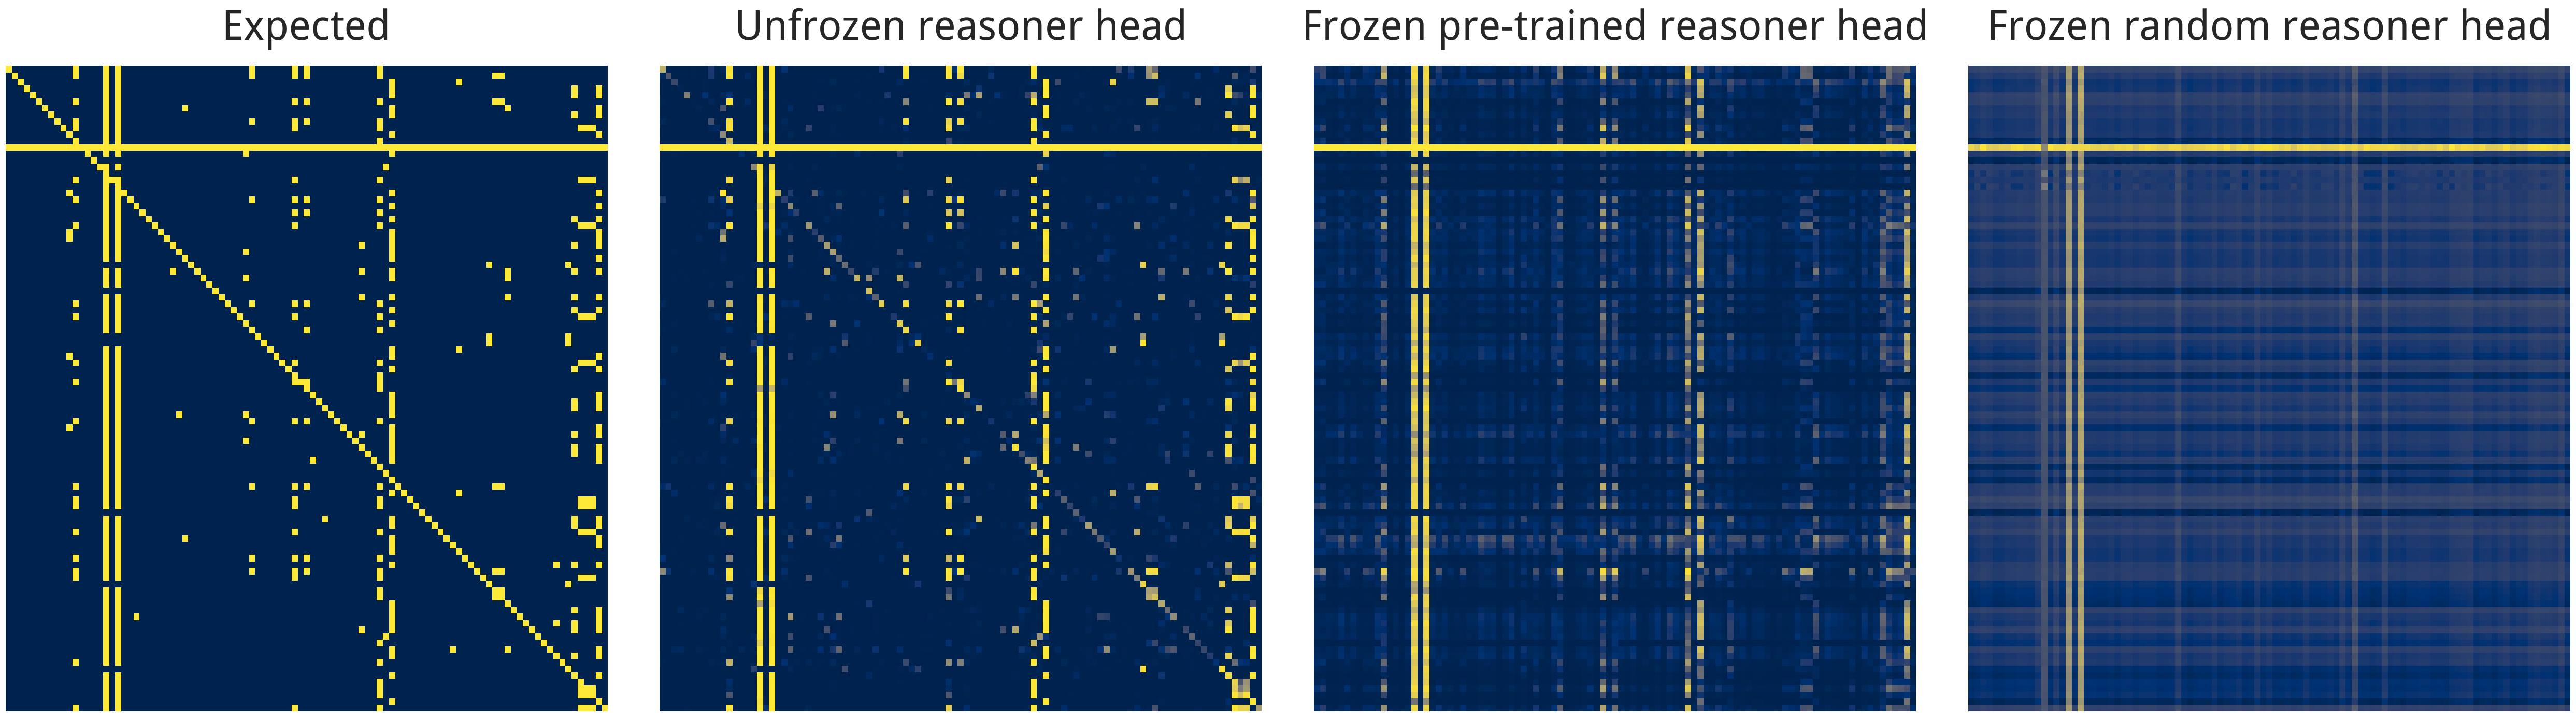
\includegraphics[width=1.15\textwidth]{figures/ex4-heatmap.png}
}
\caption{
Expected ontology classification and classification heat maps obtained with the reasoners in experiment~3.
The expected classification is the same as in~\autoref{fig:pizza-heatmap}, and is the ideal result.
We do not show the concept names, because they are not necessary for comparing heat maps.
A concept that is subsumed by every concept (a concept equivalent to $\bot$) is shown as a yellow horizontal line, and a concept that subsumes every concept (a concept equivalent to $\top$) is shown as a yellow vertical line.
}
\label{fig:ex4-heatmap}
\end{figure}

\subsection{Evaluation of knowledge transfer}

In the last section we discussed the differences between the three reasoners that we trained in experiment~3.
Taking into account the differences between the reasoners with frozen heads, we conclude that the transfer of knowledge from the randomly generated KBs in experiment~1 to the pizza ontology was a success.
The reasoner with the pre-trained head achieved similar results to the unfrozen reasoner, which is very promising, given that the pizza ontology is certainly different from the randomly generated KBs used as the training data set in experiment 1.

It should be mentioned that the total training time of the reasoners with frozen heads is approximately 17\% shorter than the training time of the unfrozen reasoner.
The training time is shorter because there is no time spent on updating the reasoner head weights.
The differences may be small at this scale, but for reasoner heads with many more parameters, transfer learning may save a lot time.

\subsection{Embedding analysis}

The last part of this experiment is to assess the UMAP visualizations of the embeddings learned by the three reasoners.
The UMAP visualizations of the learned embeddings are shown in~\autoref{fig:ex4-emb}.

We set the UMAP parameters in the same way as in experiment~2.
We kept the \tw{n\_neighbors} set to 50, to emphasize global structure, and set \tw{min\_dist} by starting at a large value and decreasing it until clusters started to separate and the visualization became readable.
The \tw{min\_dist} parameter is set to 0.2, 0.6, and 0.2 for the visualizations for the unfrozen reasoner, the reasoner with the frozen pre-trained head, and the reasoner with the frozen random head, respectively.
The larger \tw{min\_dist} value was needed for the pre-trained reasoner head, because the cluster of pizzas and the cluster of toppings were so tightly-packed, that the visualization was not readable.

The visualization of embeddings learned by the unfrozen reasoner is very similar to the visualization in experiment~2.
The data set in this experiment contained complex axioms with concept expressions using constructors, so the resulting embeddings should capture the ontology semantics better than the embeddings learned in experiment~2.
However, we admit that we do not see meaningful differences between this visualization and the one in the previous experiment.

The embeddings learned by the reasoner with the pre-trained head look a bit worse than those of the unfrozen reasoner.
The pizzas and the toppings are separated, but inside of the topping cluster the embeddings are not as well organized.
For example, some meat toppings are close to vegetarian toppings, and neither meat, nor seafood topping form their own cluster.
The cheese toppings are also scattered throughout the topping cluster.
Inside the pizza cluster, the cheesy pizzas and vegetarian pizzas are close to each other, which is good.
The named vegetarian pizzas are a bit too close to the non-vegetarian pizzas, but this may be because all of these pizzas are cheesy pizzas (except \tw{Frutti\-Di\-Mare}).
The levels of spiciness form a little cluster, which is also good. 
The top concept is close to \tw{Food} and \tw{Domain\-Thing}, which is expected, but it is also close to \tw{Cheesy\-Vegetable\-Topping}, which should be close to the bottom concept instead.
We also think that \tw{Herb\-Spice\-Topping} is too close to the bottom concept.

The embeddings learned by the reasoner with the randomly initialized head look very bad when visualized.
Very few concept names form clusters that make sense, and most look like they are randomly scattered.
In the upper left corner, a couple of cheesy vegetarian pizzas form a cluster.
In addition, general concepts are also close to the top concept, which is good.

In general, we think that the embeddings for the unfrozen reasoner are the best, the embeddings for the reasoner with the frozen pre-trained head are good, and the embeddings for the reasoner with the frozen randomly initialized head are not good at all.
Again, the results of the visual assessment of the learned embeddings are consistent with the classification metrics of the reasoners.

\begin{figure}
\makebox[\textwidth][c]{
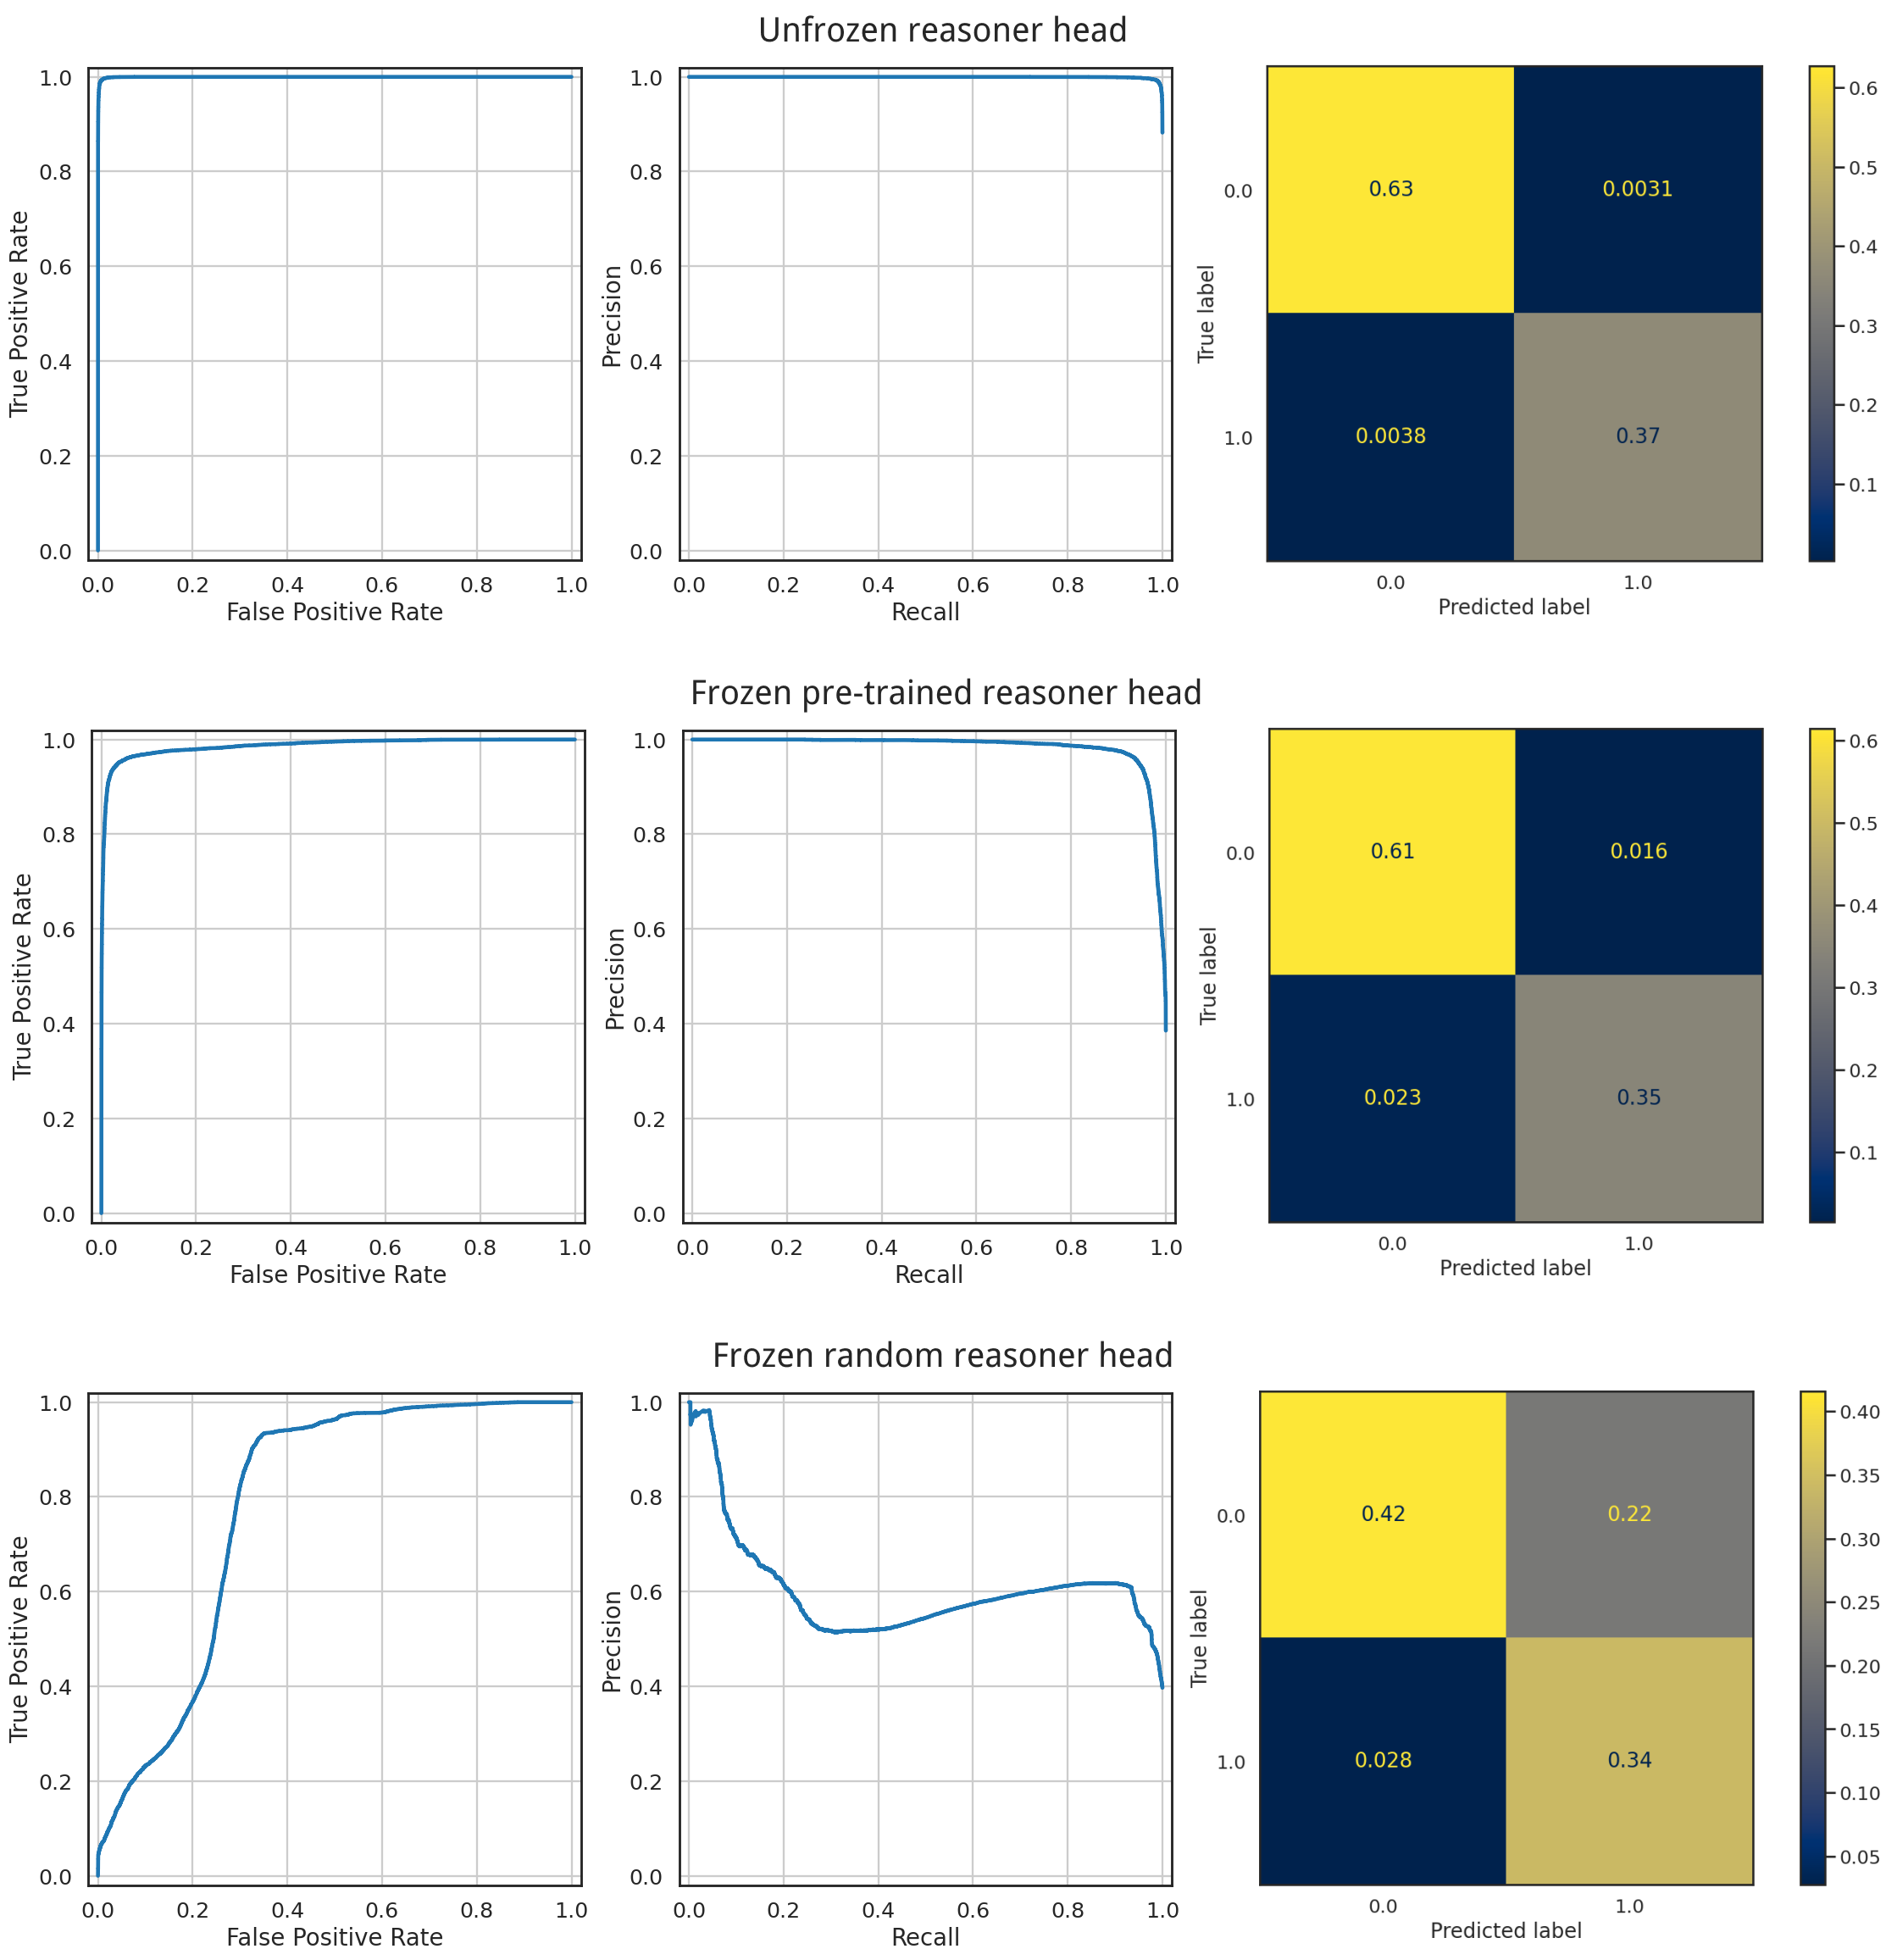
\includegraphics[width=1.15\textwidth]{figures/ex4-vs.png}
}
\caption{
ROC curves, PR curves, and confusion matrices of reasoners in experiment~3.
Confusion matrices are normalized by the number of all samples in the training data set.
}
\label{fig:ex4-vs}
\end{figure}

\begin{figure}
\vspace*{-0.5cm}
\makebox[\textwidth][c]{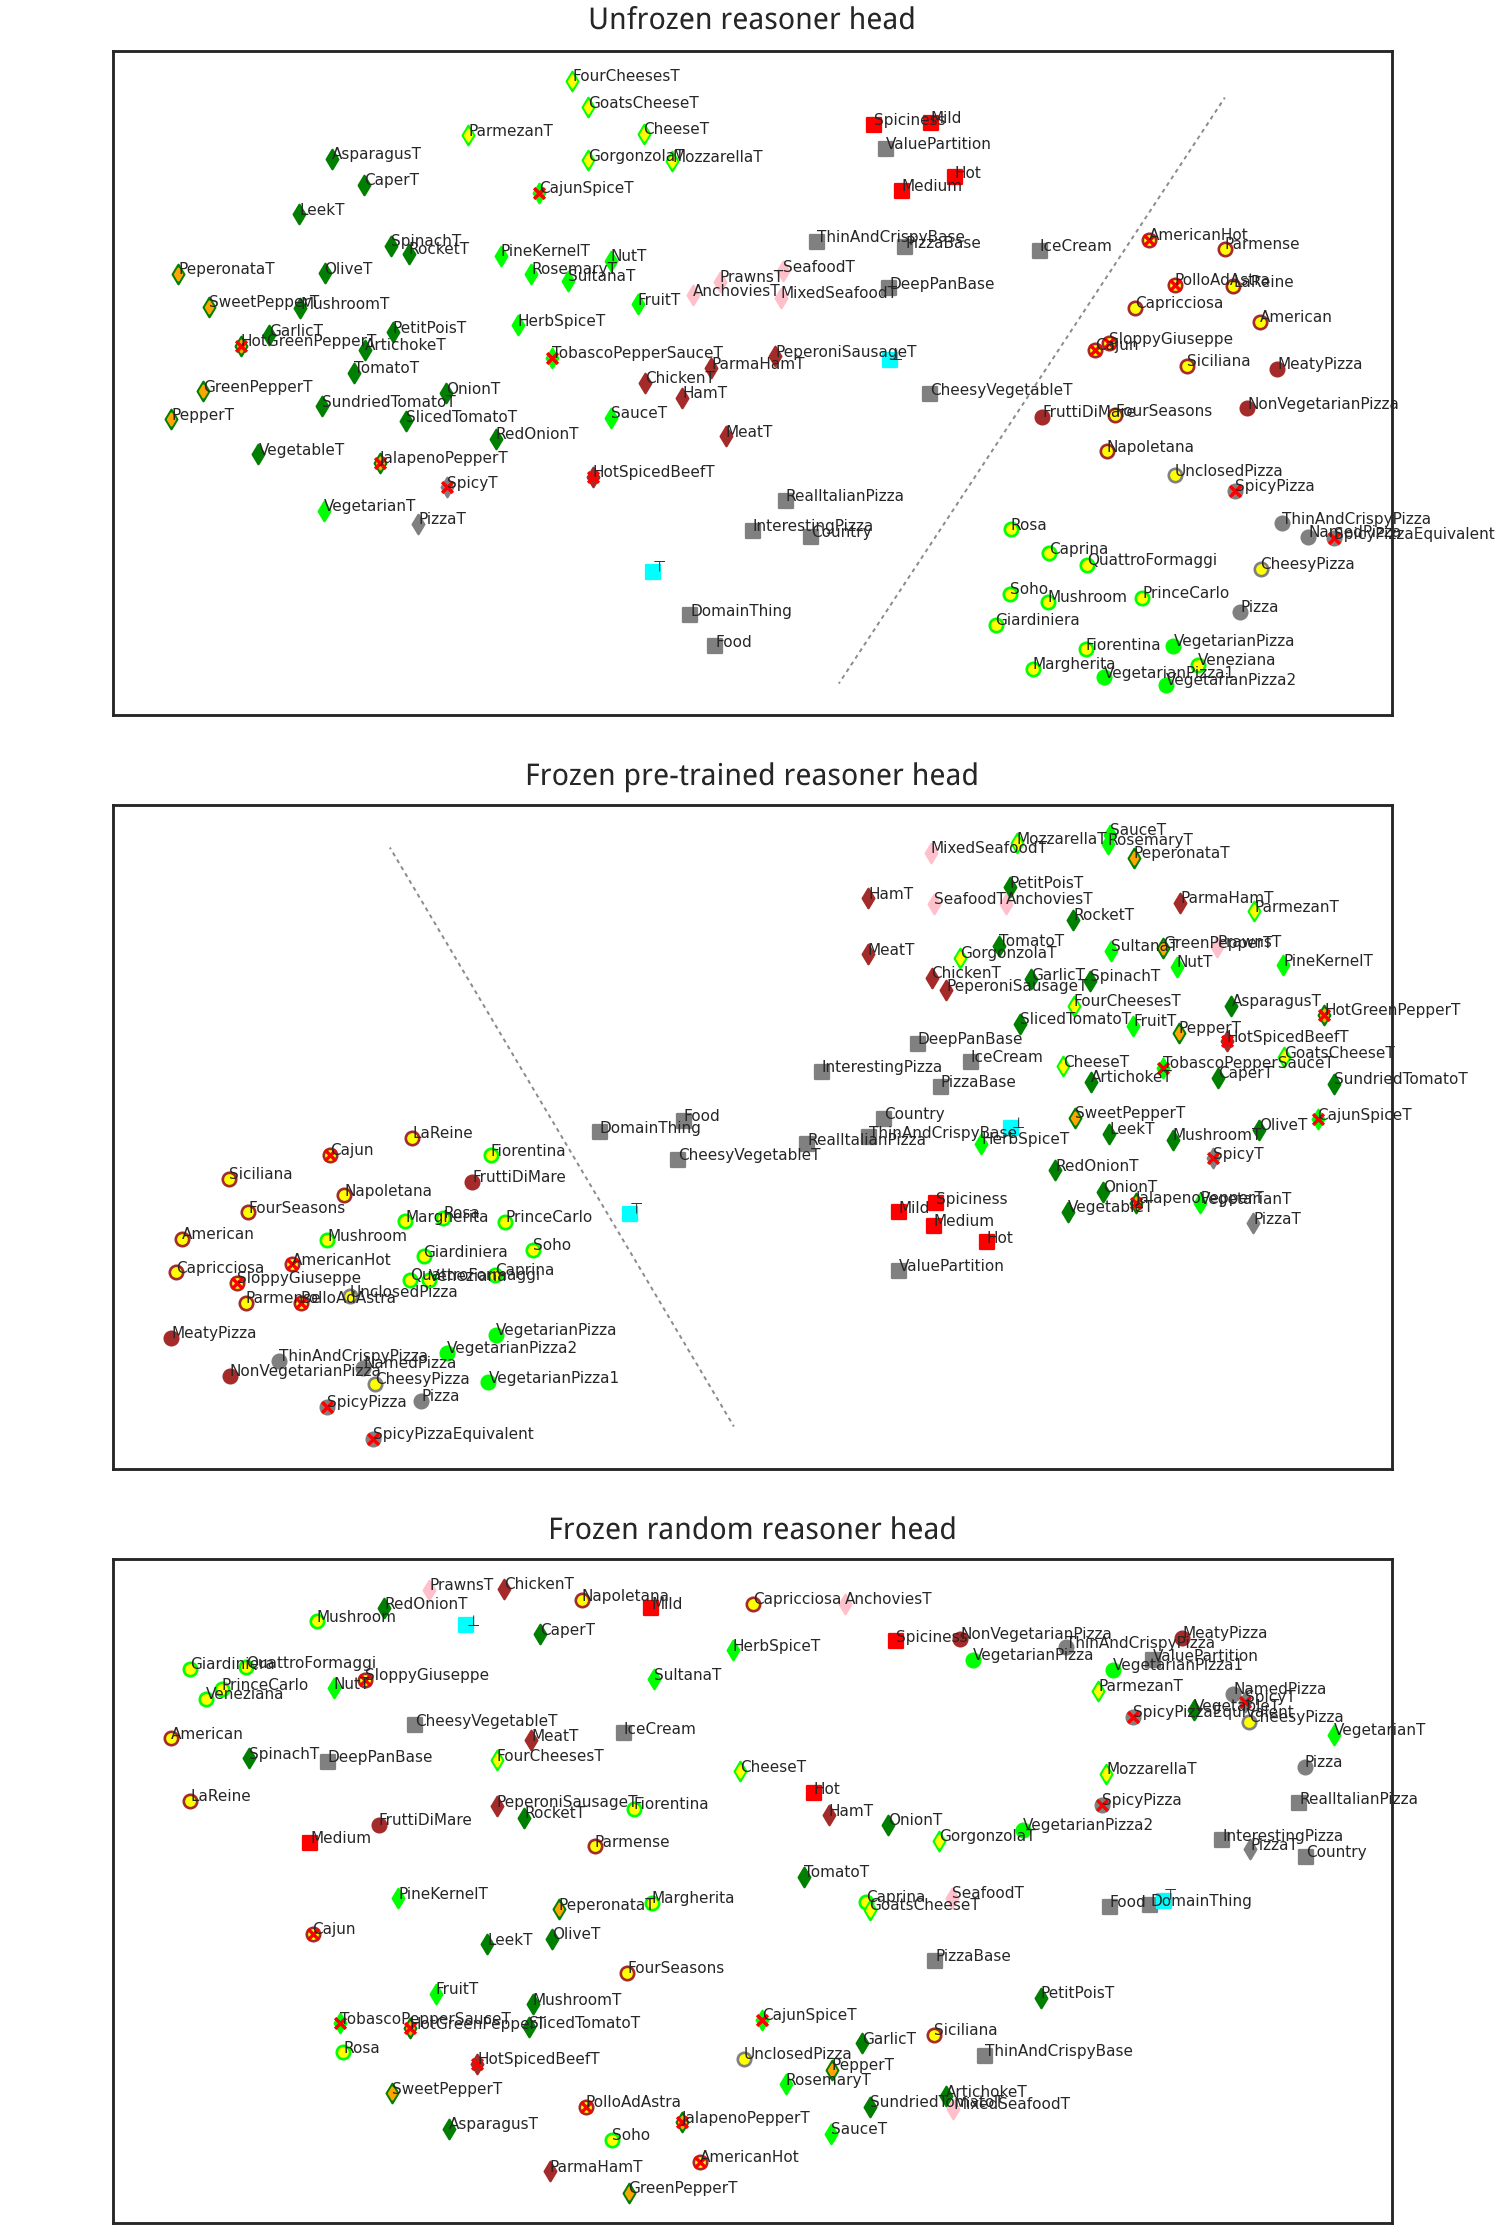
\includegraphics[width=1.125\textwidth]{figures/ex4-emb.png}}
\caption{UMAP visualizations of embeddings learned by reasoners in experiment~3. For emphasis, we added a dashed line separating pizzas and other concept names in visualizations where the two are clearly separated.}
\label{fig:ex4-emb}
\end{figure}


\chapter{Conclusions}
\label{sec:conclusions}

In our work we introduced a novel method of learning data-driven concept embeddings in $\ALC$ knowledge bases.
To our best knowledge, our method of learning concept embeddings is the first one using an entailment classifier based on deep neural networks.
Thanks to our unique approach, after learning embeddings, one can use the resulting classifier to perform fast approximate reasoning.

We also show that using recursive neural networks for constructing embeddings of arbitrarily complex concepts obviates the need for manually designing concept vectorization schemes, and avoids the pitfalls of recurrent neural networks operating on a textual representations of concepts.
Instead, concept embeddings can be learned in a data-driven way, by simply asking entailment queries for a given knowledge base.

Finally, we show that a significant part of our reasoner is transferable across knowledge bases in the $\ALC$ description logic, including small real-world knowledge bases like the pizza ontology.
The advantage of a transferable reasoner is that learning concept embeddings takes less time, and thus is less expensive, when using a pre-trained reasoner head, compared to training an entire reasoner from scratch.
Promising initial results in the transferability of deep neural reasoners suggest that it is indeed feasible to embed concepts from multiple domains in a single shared embedding space.

We hope that our deep neural reasoner architecture will allow for greater use of knowledge in models based on neural networks, both by providing an effective way of learning concept embeddings, and learning an accurate entailment classifier for knowledge bases in description logics.
Thus, making a small step towards the integration of the neural and symbolic paradigms in artificial intelligence.

\section{Further work}
\label{sec:further-work}

We identified many opportunities to improve, extend and apply our deep neural reasoner, that were out-of-scope for this work, but look like promising avenues for further research.

In our work we used small neural networks, but deeper and wider concept constructor networks, and subsumption entailment classifier networks could be examined.
The number of parameters in the reasoner could also be reduced, while preserving the quality of embeddings and accuracy of entailment classification.
Currently, the number of parameters scales quadratically with the embedding dimension, because the reasoner uses the outer product of embeddings as an input to neural networks $\nn_\sub$ and $\nn_\dland$.
Instead of passing the entire interaction map as input, convolutional neural networks could be used instead, which could greatly reduce the number of parameters.
The number of parameters used by existential restriction constructor networks could possibly be reduced by representing weights as sparse matrices.

Examining reasoner variants for other description logics like $\EL$, or extending our reasoner to support ABox reasoning might be beneficial.
It would also be worthwhile to examine how the reasoner performance scales with the embedding dimension $N_e$, and how it performs for real-world knowledge bases of different sizes, for example SNOMED CT.
After checking if deep neural reasoners can work with large real-world KBs, one could see if using learned embeddings as additional model inputs in other machine learning tasks can improve results.

Finally, it would be interesting to see if recursive neural networks could be applied in reverse to how we use them -- to generate concepts, given learned concept embeddings.
That would make it possible to not only learn concept embeddings by classifying entailment, but also to induce new concepts by sampling the embedding space.
Among other uses, concept induction can be used for explainable AI, but current algorithms are not scalable~\cite{sarker_efficient_2019}.
If it were possible to traverse the space of concept embeddings, with the gradient descent algorithm for example, then applying concept induction for explainable AI could be made feasible.
Of course this is just a vague idea of what may be possible with a bidirectional mapping between concept expressions and the concept embedding space.

\section{Acknowledgments}

We would like to thank out supervisor, dr~inż.~Jędrzej~Potoniec, for the idea of using a transferable classifier as a means for learning concept embeddings for knowledge bases in description logics, and their support and incredibly helpful discussions. We would also like to thank dr~hab. inż. Agnieszka~Ławrynowicz, our mentor in the ``AI Tech'' project, for guidance and support in our studies, and helpful feedback on our work.